%+++++++++++++++++ April
	\section{Introduction}
	
	
In this study, two different SEA designs have been implemented and tested. The first design is based on a linear movement (constrained by a linear guideway), where the rotary motion of the motor is driving a lever, pushing the carriage back and forth. For more details, see figure \ref{fig:actuation_system_explained}. \\
The second design is an approximated linear motion, due to a very large lever (rotational-L) actuated by a cam principle.
	
	\section{Design and Analysis}
	\subsection{Series Elastic Actuators}
	
		
	\subsection{Design of the PlayStation Controller}
	
	
	
	\subsubsection{Design of the Pilot Controller}
	The 3D model of the left-hand side pilot-based controller can be seen in figure \ref{fig:left_hand_joystick_cam}. To see the inside of the controller, the cover has been removed. To assemble it three sets of screws and nuts are necessary, making it easy to assemble and take apart. Also, this design is smaller in volume than the PlayStation controller. It is therefore more slender, cheaper and faster to manufacture.
	\begin{figure}[h!]
		\centering
		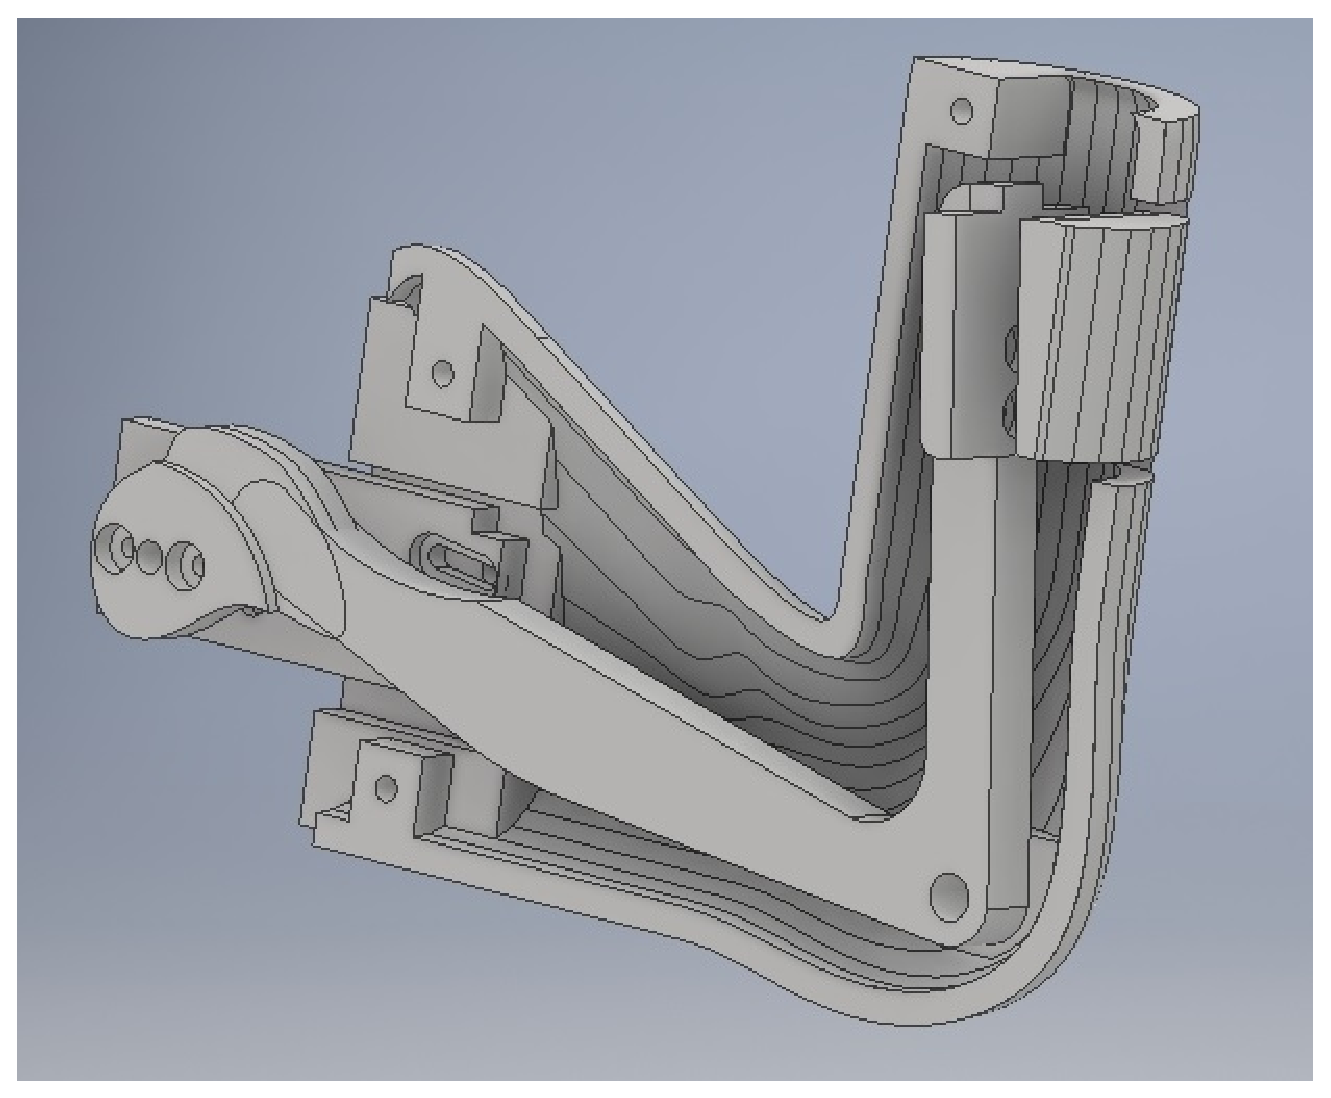
\includegraphics[width=0.4\linewidth]{Figs/left_hand_joystick_cam}
		\caption{3D model of the left-hand side controller with a removed cover.}
		\label{fig:left_hand_joystick_cam}
	\end{figure}

	In this design, the feedback motion is perpendicular towards the user and opposing the direction of motion. However, there is a slight angle at which the force is acting, due to the rotational design in the controller. But due to the large lever, this effect can be neglected. The actuation principle is based on a simple cam disk that directly pushes the rotational-L. For this design, the motors with a higher reduction gear ratio have been foreseen.
	
	
	\subsection{Test Environment and Programs}
	To test the controller, it was necessary to write a properly working environment. The topy robot is communicating via a wireless serial link. It has a prespecified communication message that consists in $70$ bytes for sending from the robot to the PC and $44$ bytes for message to receive. These messages include the bytes reserved for proper starting and ending as well as the checksum. \\
	It was thus necessary to write an application that reads out the position of the two joysticks (basic potentiometers principle) and construct a message including these joystick values as speed reference for the robot. Then the message has to be sent over the wireless serial link to the robot and the answer has to be received. The important sensor readings (inclination, current in the crawlers, passed time and battery level) have to be read out and a feedback according to the chosen feedback law has to be sent to the motors.\\
	For this purpose, the programming language processing \footnote{\url{https://processing.org/}} has been used to create a graphical user interface and to establish the serial connection. For low-level motor control purposes an Arduino Uno has been used. The parameters that can be set for testing purposes can be seen in table \ref{tab:programming_params}.
	
	\begin{figure}[h!]
		\centering
		\begin{tabular}{|l|c|l|}
			
			\hline
			Setting & Value & Units \\ \hline \hline
			Baud rate for robot serial link & $9600$ & [bps]\\ \hline
			Baud rate for Arduino serial link & $9600$ & [bps] \\ \hline
			Update rate of the processing GUI & $5$ & [Hz] \\ \hline
			Update rate of the Arduino motor controller (in theory) & $200$ & [Hz] \\ \hline
			Update rate of the Arduino motor controller (in practice) & $170$ & [Hz] \\ \hline %TODO this should be in measured not in set parameters
			Max voltage for motor & $20$ & [V] \\ \hline
			Feedback resolution & 5 out of 255 & [-] \\ \hline
			PWM frequency & $31372.55$ & [Hz]  \\ \hline
			Proportional motor gain & $1.5$  & [-] \\ \hline
			Integral motor gain & $0.0$  & [-]\\ \hline
			Derivative motor gain & $0.0$  & [-]\\ \hline
			Feedback filter  & $50$ & [\%] \\ \hline %TODO calculate cut off frequency
			Left photoreceptor MIN value & $500$ & [-] \\ \hline %TODO explain more in detail what these values mean
			Left photoreceptor MAX value & $770$ & [-] \\ \hline
			Right photoreceptor MIN value & $680$ & [-] \\ \hline
			Right photoreceptor MAX value & $770$ & [-] \\ \hline			
		\end{tabular}
		\caption{Software parameters.}
		\label{tab:programming_params}
	\end{figure}
	
	\subsection{GUI in Processing}
	The graphical user interface shows the current feedback method as well as the magnitude. It also indicates which driving direction (forward, backward or halt) is sent to the robot. Since there is no control of the battery charge in the robot, it sends battery information in its message to the PC. The processing program reads out the charge of the battery and warns the user if it is too low. It stops the program, if the battery state is critical. The feedback method can be changed by a mouse-click anywhere in the window. The GUI can be seen in figure \ref{fig:processing_gui}.
	 
	\begin{figure}[h!]
		\centering
		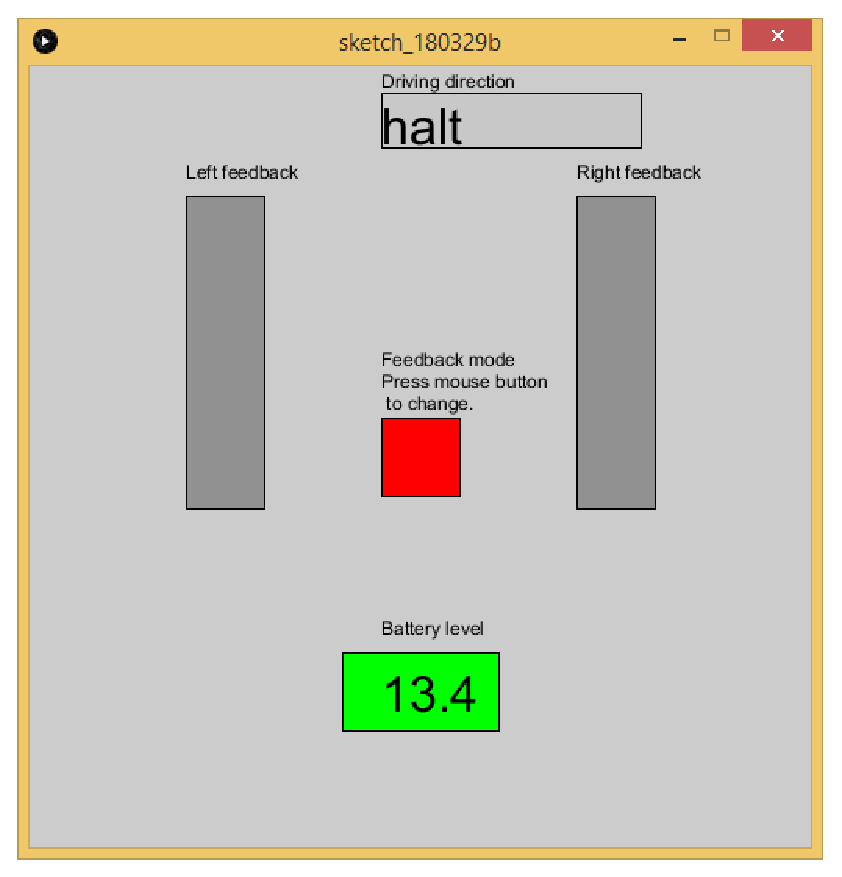
\includegraphics[width=0.4\linewidth]{Figs/processing_gui}
		\caption{Graphical user interface written in processing.}
		\label{fig:processing_gui}
	\end{figure}

	This application handles the messages sent to and from the robot.
	
	\subsection{Control Scheme}
	The control scheme is based on a simple proportional controller. The scheme can be seen in figure \ref{fig:control_scheme}. In the test setup the reference signal $dist_{ref}$ is given by the sinusoidal function generator. In the operational mode, this corresponds to the target output force, also called the haptic feedback force that should be felt by the user. Ideally, this shall be a function of orientation (roll and pitch) as well as the current in the two crawlers.
%deleted figure and put it in chapter playstation design
	
	\subsection{Electrical low-pass Filter}
	Before the PWM signal from the Arduino is sent to the amplifier, where it is amplified to control the motors, it has been filtered with a simple RC low-pass filter. The resistor has a value of $3.9$ k$\Omega$ and the capacitor of $0.1$ $\mu$F. This smooths out the PWM signal and has been implemented in order to avoid that the amplifier tries to follow the Arduino signal with unnecessary precision, eventually causing too much heat.
	
	
	\subsection{Photoreceptor Circuit}
	The photoreceptor that has been used is the TPR-105 from GENIXTEK CORP. Its sensing characteristics can be seen in figure \ref{fig:photoreceptor_curve}. The electrical circuit can be seen in figure \ref{fig:tpr105_circuit}. The component values are $R_1 = 330 \Omega$, $R_2 = 62$k$\Omega$ and $V_{CC} = 5$V. This receptor returns a $10$-bit value.
	
	\begin{figure}[h!]
		\centering
		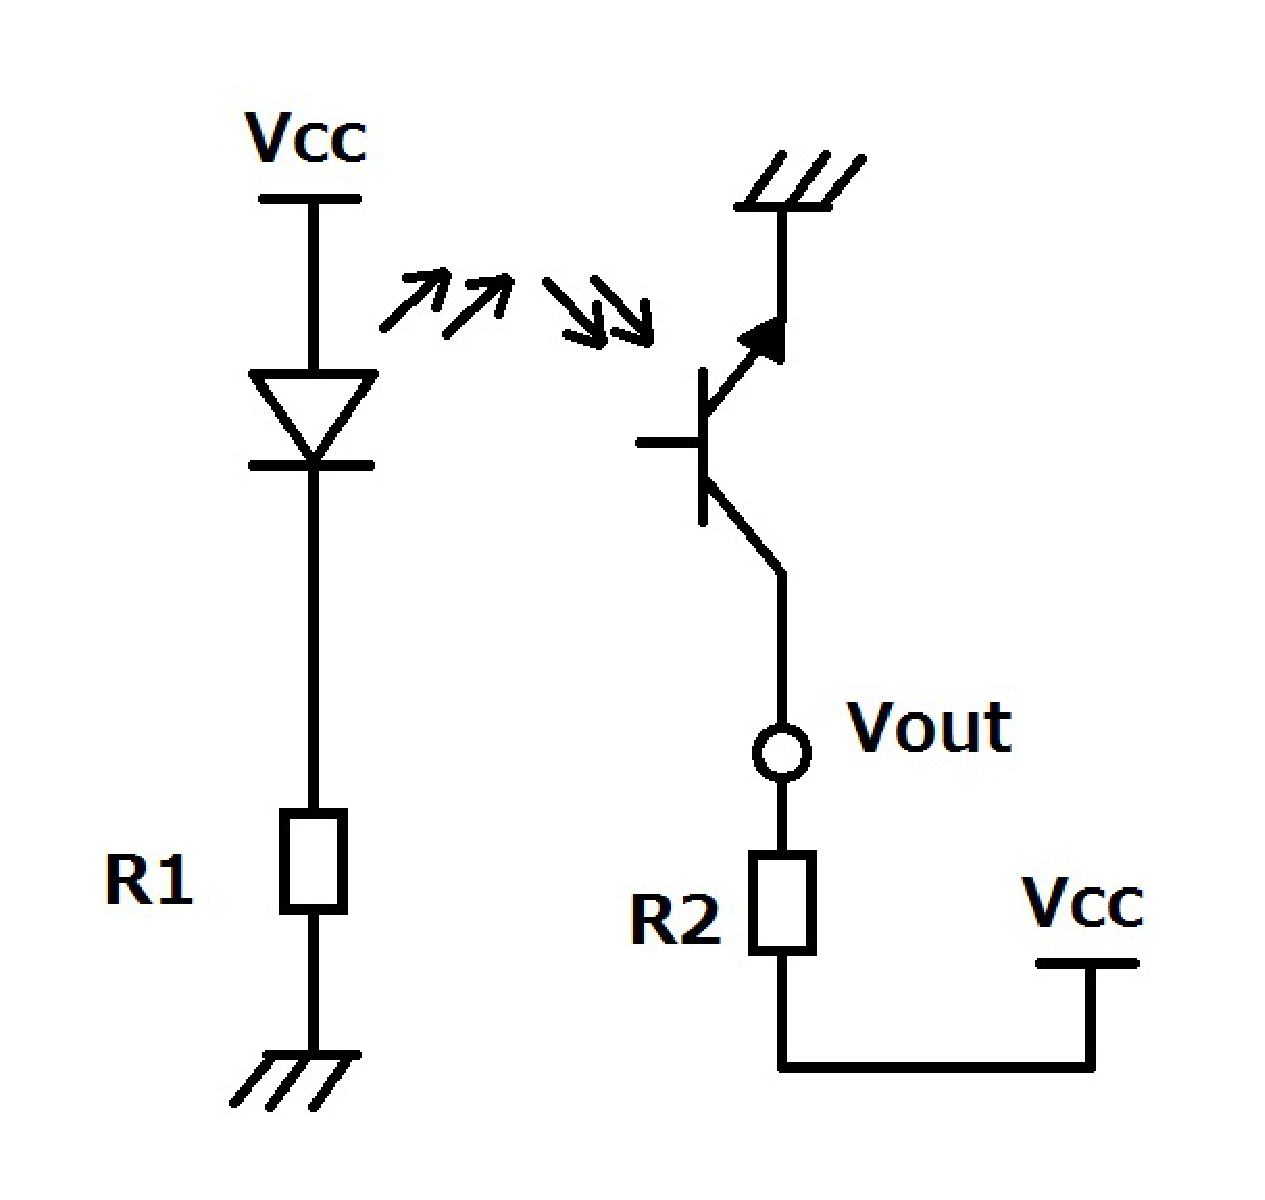
\includegraphics[width=0.2\linewidth]{Figs/tpr105_circuit}
		\caption{Implementation circuit of the photoreceptor.}
		\label{fig:tpr105_circuit}
	\end{figure}
	\begin{figure}[h!]
		\centering
		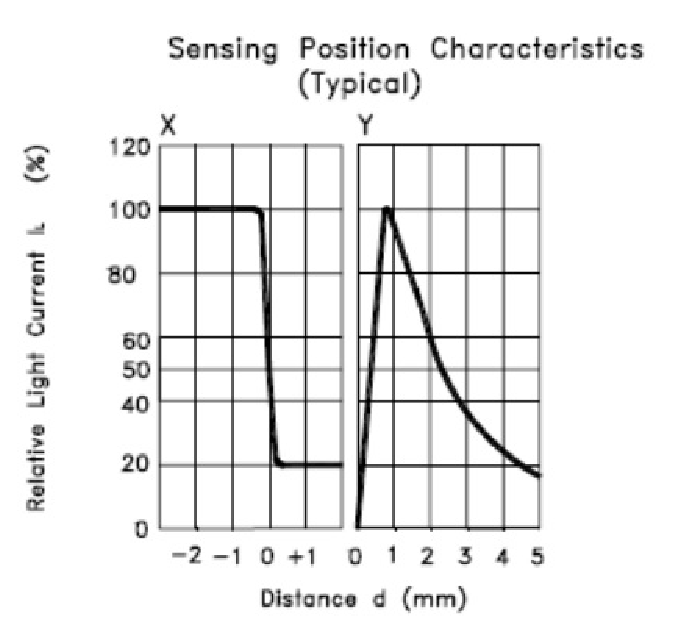
\includegraphics[width=0.3\linewidth]{Figs/photoreceptor_curve}
		\caption{Sensing characterstics of the photoreceptor TPR-105. Taken from its datasheet.}
		\label{fig:photoreceptor_curve}
	\end{figure}

	The sensing characteristics shows a nonlinear function in the range between $1$mm and $5$mm. However, as a first step, this has been interpolated linearly. To put it more precisely, the target output force has been mapped linearly to the measured distance. The operational distance lies between $4.5$mm to $5.5$mm.
	
	\section{Testing of the PlayStation Controller}
	For the two sides of the controller two different spring constants have been used. On the left-hand side, there is a set of three springs with a constant of $0.98$N/mm each. The motor has a reduction gear ratio of $33:1$. On the right-hand side the springs have a constant of $9.8 $N/mm and the motor has a reduction of $112:1$. The parameters are resumed in table \ref{tab:playstation_charac}.
	
	\begin{figure}[h!]
		\centering
		\begin{tabular}{|l|c|c|l|}
			\hline
			& Left side & Right side & Units\\ \hline \hline
			Clamp link length & 20 &  20 & [mm]  \\ \hline
			Motor reduction & $33:1$ & $112:1$ &  [-] \\ \hline
			Output torque (continous) & $30$ & $93$ & [mNm]  \\ \hline
			Output torque (intermittent) & $100$ & $180$ & [mNm] \\ \hline
			Number of springs used & $3$ & $3$ & [-] \\ \hline
			Spring constant & $0.9$ & $9.8$ & [N/mm] \\ \hline
			Equivalent spring constant & $2.7$ & $29.4$ & [N/mm] \\ \hline
		\end{tabular}
		\caption{Motor setup characteristics}
		\label{tab:playstation_charac}
	\end{figure}

	In order to conduct the frequency response analysis, the SG-4115 Function Generator has been used. The output signal was a sine wave with a peak-to-peak value of $2$V and an offset of $1.4$V. These settings have been made in order to stay within the detectable range of the Arduino $[0..5]$V. The frequency has been varied between $0.1$Hz and $35$Hz with $20$ logarithimcally spaced steps.
	
	Since the palm pads are blocked by the users hand in operational mode, they may not be considered blocked by an infinitely stiff wall. Therefore two different test setups have been created, where the palm pad has first been blocked by a screw driver in both directions, to have close to infinite stiffness, and a second setup, where the palm pads have been blocked by the users hands.
	
	\subsection{Results for Fixed Palm Pad Experiment (Pseudo Infinite Stiffness)}
	The input signal has been received as a feedback value (ie. $dist_{ref}$) and the P-controller stated in table \ref{tab:programming_params} controlled the output force by linearly mapping it to the photoreceptor distance. The measured distance has been logged and plotted. As it was expected, it is between the two extreme values stated in table \ref{tab:programming_params} (MIN and MAX). The response for the two extreme frequencies can be seen in figure \ref{fig:resp_left_hand_rigid_experim1}.
	\begin{figure}[h!]
		\centering
		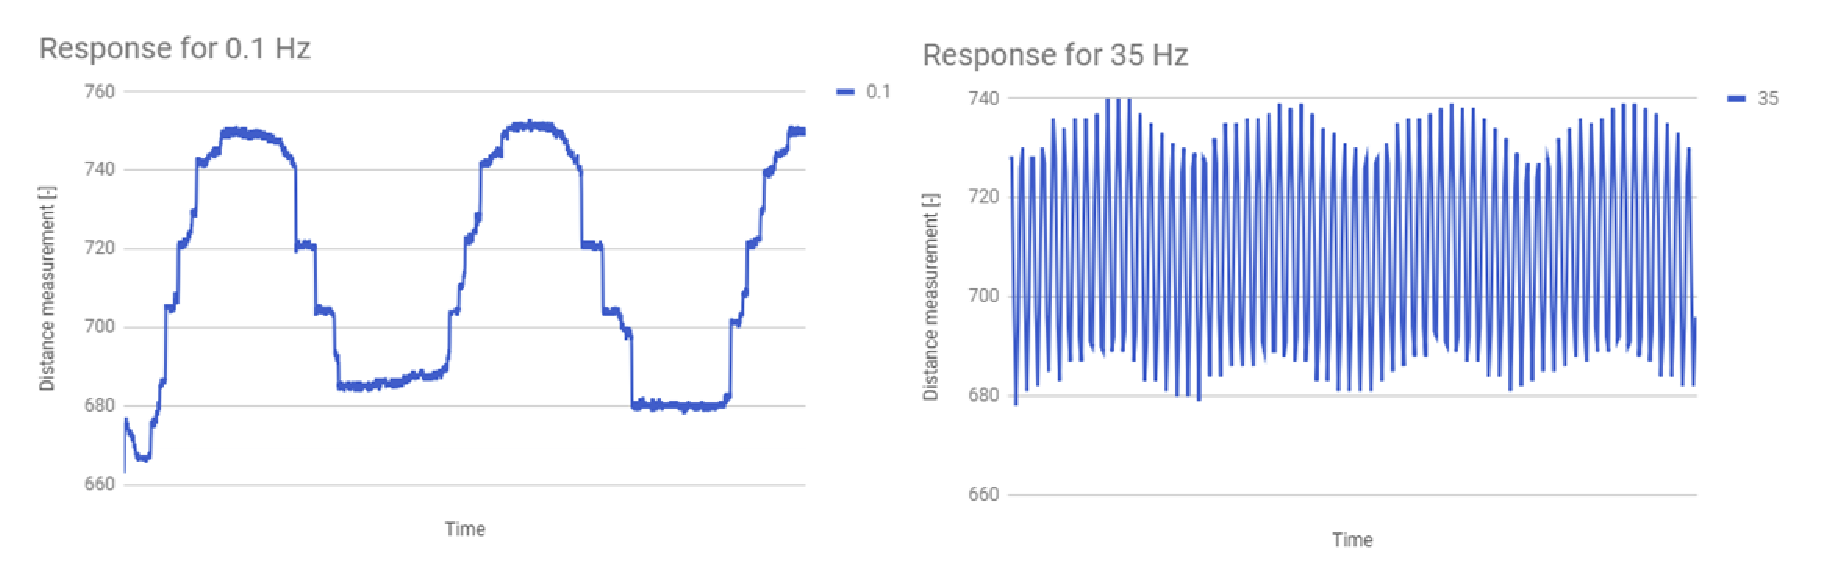
\includegraphics[width=0.7\linewidth]{Figs/resp_left_hand_rigid_experim1}
		\caption{}
		\label{fig:resp_left_hand_rigid_experim1}
	\end{figure}
	
	In order to find the frequency response, one is interested in the amplitude correlation between the input signal and the output signal, as given in the following equation:%TODO write how the FRF can be found, find a paper and reference it
	\begin{equation}
		H = \frac{F^*(j\omega)}{F(j\omega)}
	\end{equation}
	Where $F^*(j\omega)$ is the transfer function of the output signal and $F(j\omega)$ of the input signal.\\
	To calculate the amplitude of the output function (the measured value by the photoreceptor, corresponding to the distance between sensor and palm pad) one should ideally have a distinguishable value which is given by the maximal and minimal value of the sinusoidal output function. However, due to noise in the system, a sometimes occurring drift, interpolation aliasing and other effects such as the plateau characteristics shown in figure \ref{fig:resp_left_hand_rigid_experim1} and discussed in a later section, these minimum and maximum values are not clearly defined. Therefore, two different approaches have been chosen for the pseudo infinitely blocked palm pad experiment.
	
	First, the two quartile values ($Q_1$ and $Q_3$) have been calculated based on all the data, including outliers and noise. This is a relatively time-efficient method and is supposed to be less accurate since it sometimes includes errors such as the initial downward spike shown in the figure \ref{fig:resp_left_hand_rigid_experim1} for $0.1$Hz. The difference between these two quartile values has then been divided by the difference of the quartiles of the input signal ($Q_{3(sine)} - Q_{1(sine)}$). The results are indicated by the blue lines in figure \ref{fig:freq_resp_both_hands_rigid_experim1}.
	
	
	\begin{figure}[h!]
		\centering
		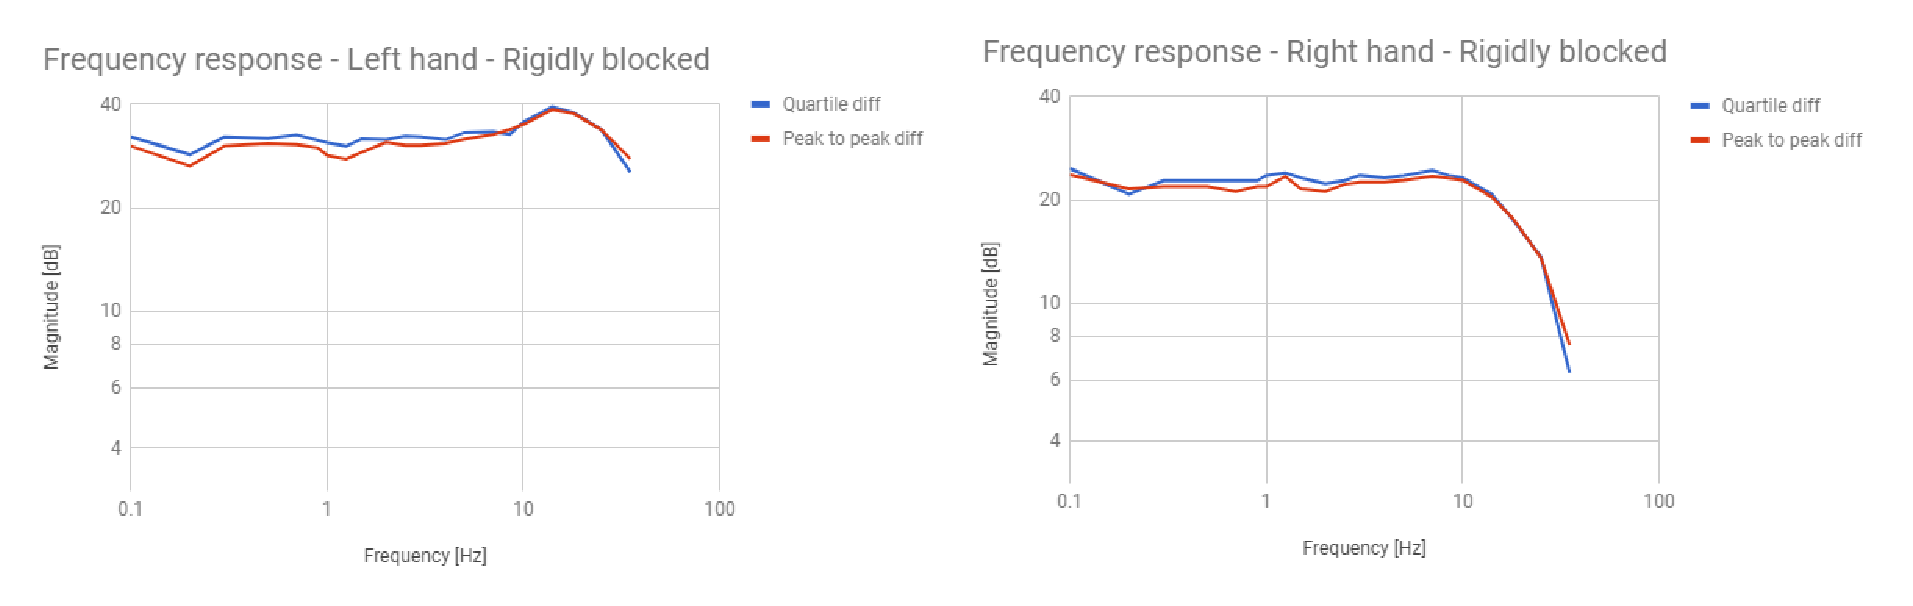
\includegraphics[width=1\linewidth]{Figs/freq_resp_both_hands_rigid_experim1}
		\caption{Frequency response analysis for both hands with a pseudo infinitely blocked palm pad.}
		\label{fig:freq_resp_both_hands_rigid_experim1}
	\end{figure}

	As an alternative output function, the amplitude has been measured manually, taking an average over several minima and maxima. This method is much more time consuming, but allows for filtering the noisy parts of the measurement, since it requires a visual representation of the measured data. These values are indicated on the same figure by the orange lines.
	
	\subsection{Results for Hand-Blocked Palm Pads Experiment}
	In the second experimental setup, the palm pads have been blocked by the hands of the user, to simulate an environment closer to the operational mode. This time, only the quartile method has been used to calculate the amplitude of the output signal. The results can be seen in figure \ref{fig:freq_resp_both_hands_soft_experim1}.
	\begin{figure}
		\centering
		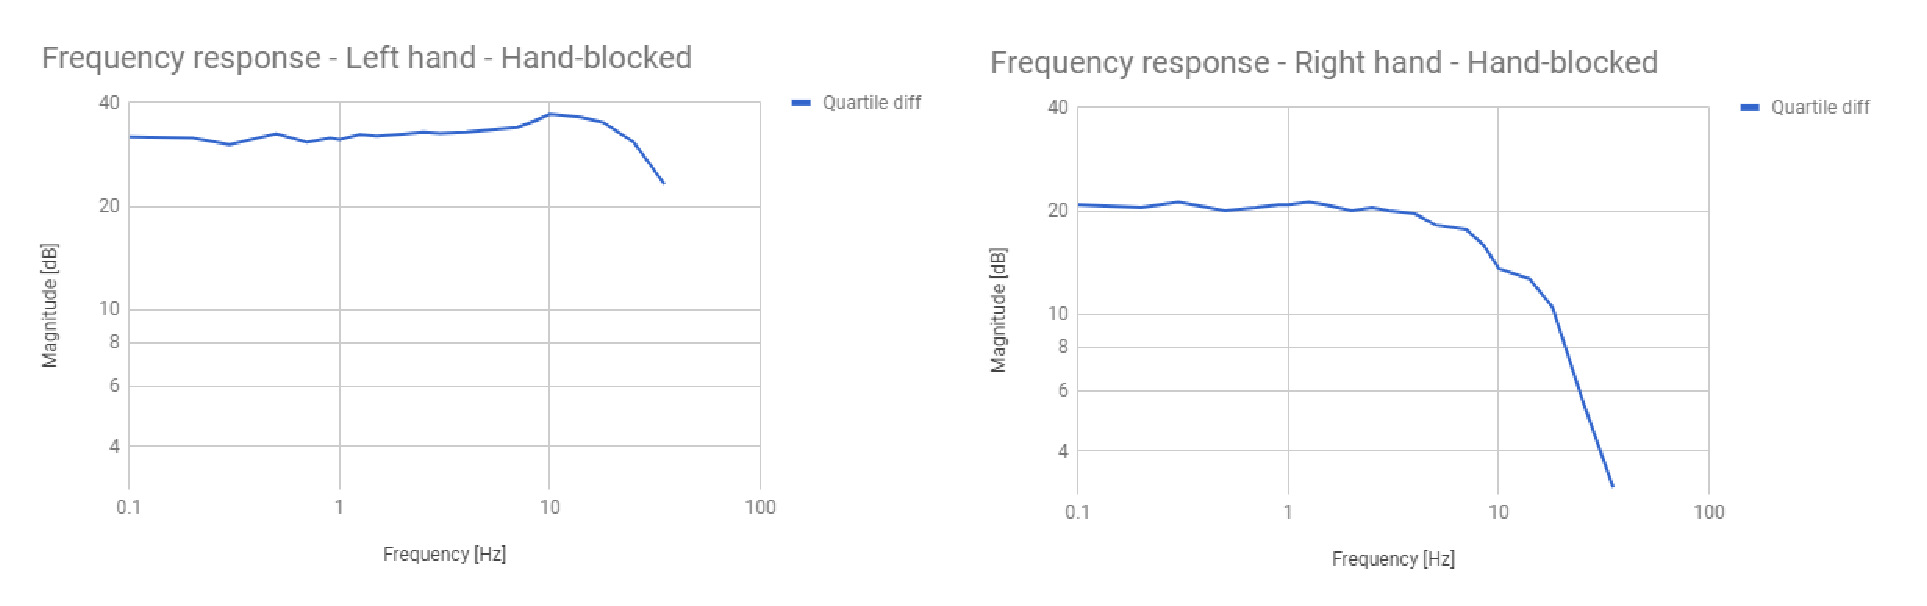
\includegraphics[width=1\linewidth]{Figs/freq_resp_both_hands_soft_experim1}
		\caption{Frequency response analysis for both hands with a hand-blocked palm pad.}
		\label{fig:freq_resp_both_hands_soft_experim1}
	\end{figure}
	
	The order of the system can be identified when looking at the slope of the Bode plot after its resonance top\footnote{Acutally, one should also consider the phase plot, but due to the reasons mentioned later in this research, this step has been skipped.}. This has been calculated for the six different curves and the following slopes have been found:
	
	\begin{tabular}{|c|c|c|}
		\hline 
		Rigid & left hand, blue line & $-54$ dB per dec \\ 
		\hline 
		& left hand, orange line & $-65$ dB per dec \\ 
		\hline 
		& right hand, blue line & $-54.8$ dB per dec \\ 
		\hline 
		& right hand, orange line & $-60.4$ dB per dec \\ 
		\hline 
		Soft & left hand & $-62.4$ dB per dec  \\ 
		\hline 
		& right hand & $-41.1$ dB per dec \\ 
		\hline 
	\end{tabular} 
	
	\section{Discussion}
	\subsection{Control Scheme and GUI}
	The control scheme is a simple proportional controller. It has been tested and decided to work well enough. If time permits, an integration and fine-tuning of an integral and derivative term can be done. \\
	There is not much to say about the GUI, however the handling of messages is not always done successfully. From time to time the processing program receives a message from the robot which is not complete. This results in accessing a cell of an array that is out of boundaries and the program crashes. To ensure the stability of the program, this case needs to be handled.
	
	\subsection{Design and Fabrication of the PlayStation Controller}
	The design of the controller is rather bulky and the actuation system might be too complex for what it is supposed to do. Due to its size, the upper and lower parts do not fit in the 3D printer and had to be cut in half and assembled by screws. This adds an extra step in manufacturing and assembly, making it more time-consuming. However the overall assembly is quite easy and tolerances have been chosen such that the whole system works. The feedback direction is not chosen optimally, if one aims at having a feedback opposing the driving direction (as seen from the robot).
	
	\subsection{Design and Fabrication of the Pilot Controller}
	This controller has almost been fully assembled, however not tested yet. It is much more simple to manufacture, as well as assemble. This design focused on having a feedback opposing the direction of motion.
	
	
	\subsection{Frequency Response Function}
	Figure \ref{fig:resp_left_hand_rigid_experim1} mainly shows two things. Firstly, there seems to be a certain step size, which is considerably more than expected. This results in only few values to attain for the photoeceptor, which can easily be seen in the response for $0.1$Hz. The second thing is, that at higher frequencies the Arduino has a too low update frequency and cannot follow the imposed sine signal, resulting in some aliasing effects. This shows that the Arduino is not capable of following frequencies higher than $35$Hz, but it also shows that the Arduino is not the right choice as a control device. The data analysis is therefore only to take with a grain of salt, since the important region after the resonance top had to be cut off. Future experiments shall be conducted using an mbed device, capable of operating at a control loop frequency of at least $1$kHz.
	
	As it can be seen in figure \ref{fig:freq_resp_both_hands_rigid_experim1} the two different methods of measuring the amplitude of the output signal share the same allures to a certain extent. This legitimizes to use the much more time-efficient approach of calculating the amplitude using the two quartile values. This argument has already been used for the data analysis in the experiment where the palm pads have been blocked by the users hand.
	
	The two figures \ref{fig:resp_left_hand_rigid_experim1} and \ref{fig:freq_resp_both_hands_rigid_experim1} show similar characteristics. Based on this, it seems appropriate to treat the two cases of pseudo infinite stiffness and hand-blocked palm pads as the same environment and for ease of analysis, only one of the two cases shall be treated.
	
	
	
	\section{Conclusion}
	The data that has been gathered with the Arduino as control device is only significant to a certain extent. The conclusions of using a screwdriver to block the palm pads for the experiments instead of the hand is still valid. However, the investigated frequency regions are too low to draw a meaningful conclusion and thus needs to be studied in more detail with a different control device (ie. an mbed). In addition to that, the phase diagrams have to be taken into account to confidently determine the order of the system.\\
	Furthermore, the most sensitive range of the photoreceptor is between $1$mm and $2$mm. The current implementation however is at a distance of roughly $5$mm making it much less linear and also less sensitive. This distance shall be reduced to increase linearity and sensitivity.
	
	
	\section{Outlook}
	First, the measured distance of the photoreceptor shall be changed to be in the range of $1.5$mm to $2.5$mm to have maximum linearity and sensitivity.\\
	The next step is to program the mbed to achieve the same control structure as with the Arduino, only with a higher control frequency. This should make it possible to study the system for higher frequencies. The control frequency shall be of $1$kHz, aiming for a maximum frequency of $100$Hz (Nyquist frequency is $f_s = 500$Hz and the practically achievable frequency is roughly one $5$th of this value).\\
	The experiments shall be conducted and analyzed again, this time also taking into account the phase plot in the Bode diagram. \\
	Additionally, the second controller shall be fully assembled and tested in the same manner.\\
	In parallel, the datasheet of the PMA servo motor driver shall be translated into English and the device integrated in the setup.

	
	%‚±‚±‚Ü‚Å
}










%+++++++++++++++++ May
	
	\section{Introduction}
	This report is the continuation of the first report about the project "Haptic Feedback Controller with Palm Pressurization". The last report has left off with the conclusion that the Arduino had a limited operating frequency and that the gathered data was not reliable enough, since not the whole region of interest in frequency could be covered. First, the idea was to use an mbed and program it to be able to replace the Arduino. However, with a few tricks %TODO explain what I did with prescaler and such
	it was possible to reduce the time of some commands to a minimum to stay at an operating frequency of $1$kHz. \\
	This report explains the setup and states the result for the adapted controller and provides a somewhat short explanation and discussion of the gathered data.
	
	\section{Experiment and Data Gathering}
	The setup can be seen in figure \ref{fig:setup_annotated}.
	\begin{figure}[h!]
		\centering
		\includegraphics[width=0.4\linewidth]{Figs/setup_annotated}
		\caption{Schematic of the spring system setup.}
		\label{fig:setup_annotated}
	\end{figure}
	For this experiment, a total of four springs, arranged symmetrical on the palmpad have been used. The springs have a spring constant of $k_s = 1.5$N/mm which corresponds to an equivalent spring constant of $k_{eq} = 6$N/mm. They are distributed around the palm pad, where in their middle a distance sensor (called photoreceptor) has been attached, to measure the distance between the L-plate and the palm pad. It therefore measures the compression of the springs, which can be related to the output force by Hooke's law as:
	\begin{equation}
		F = k_{eq}x 	
	\end{equation}
	
	\subsection{Setup}
	In this experiment a thorough frequency response analysis shall be done on the controller. On the left-hand side the motor with a reduction ratio of $33:1$ has been used, whereas for the right-hand side, the motor has a reduction ratio of $112:1$. \\
	A reference signal is fed into the Arduino, which then controls the motors to match the compression of the springs with the reference. The operational distance of the photoreceptor to the palm pads is $2$ to $4$mm which lies within the more sensitive region of the sensor.
	
	\subsection{Control Scheme}
	The reference signal is given by the Function Generator SG-4115. This generator has an intrinsic output impedance of $50$Ohm. This means, that it expects to have a device connected to it with the same value as input impedance. If this is the case, these two elements form a simple voltage divider and only half of the voltage is applied to the target device. However, this is not the case for the Arduino, since it has a considerably higher input impedance. Therefore, the settings made on the function generator result in double the voltage on the Arduino. From this point on, this issue shall be neglected and all future voltage indications refer to the voltage level as seen by the Arduino.\\
	The function generator produces a sine wave between $0$ and $5$V with a frequency ranging from $1$ to $100$Hz. The Arduino reads this voltage and controls the motor to have a proportional spring compression accordingly. In this case $0$V as reference signal is $0\%$ compression and $5$V corresponds to $100\%$ compression. The control scheme of this setup can be seen in figure \ref{fig:frf_measure_points}.
	\begin{figure}[h!]
		\centering
		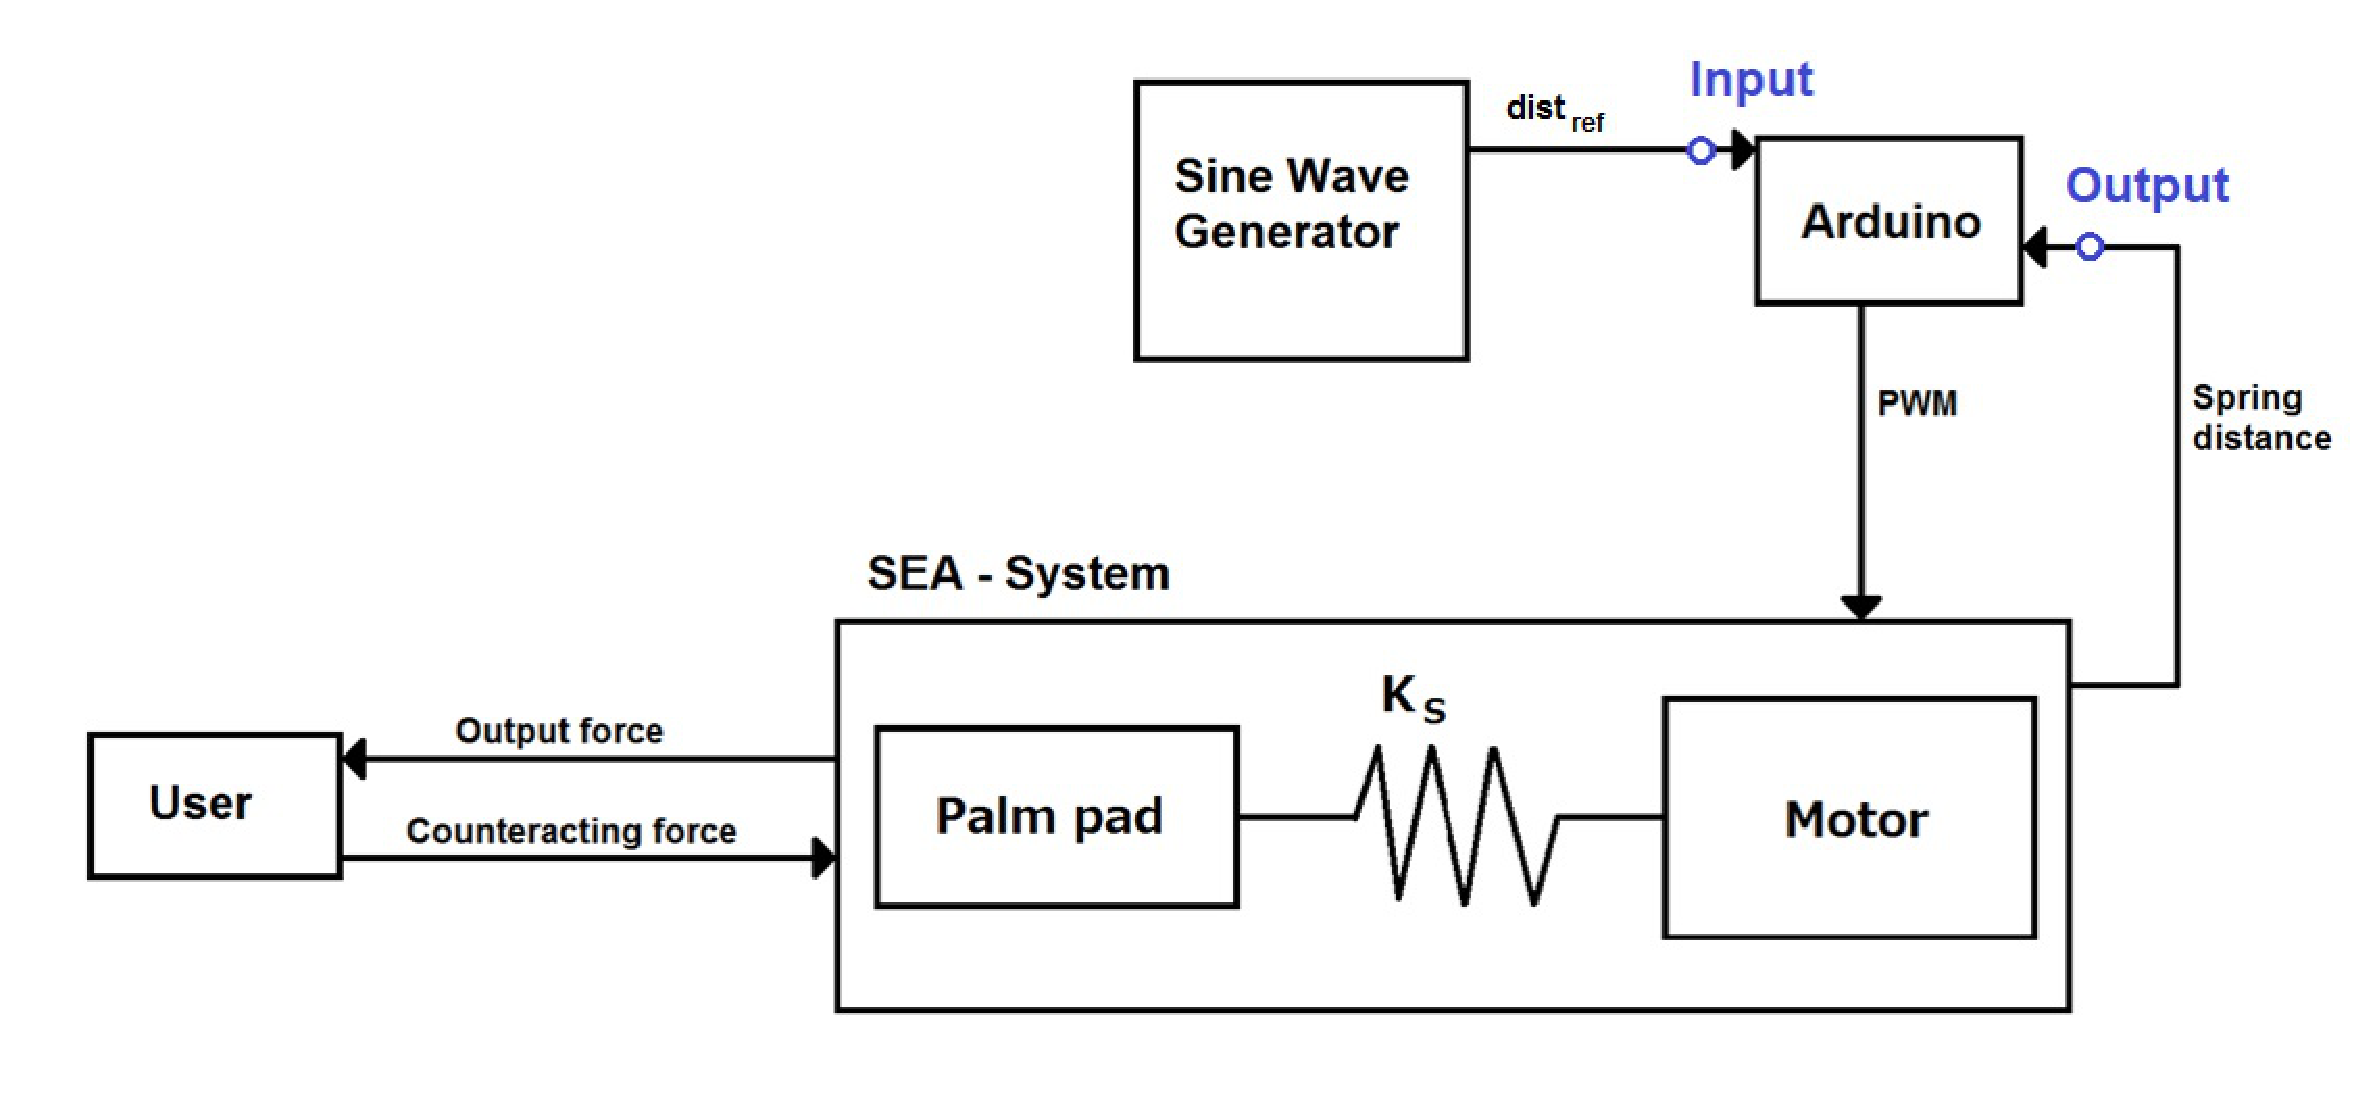
\includegraphics[width=0.6\linewidth]{Figs/frf_measure_points}
		\caption{Control scheme for the frequency response analysis.}
		\label{fig:frf_measure_points}
	\end{figure}
	In this case the counteracting force from the user is infinite, since the palm pads have been blocked by a wall.
	
	\subsection{Photoreceptor Circuit}
	The circuit of the photoreceptor can be found in figure \ref{fig:tpr105_circuit}. The components chosen are the TPR-105 for the sensor, $R_1 = 330\Omega$ and $R_2 = 27k\Omega$.
	
	\begin{figure}[h!]
		\centering
		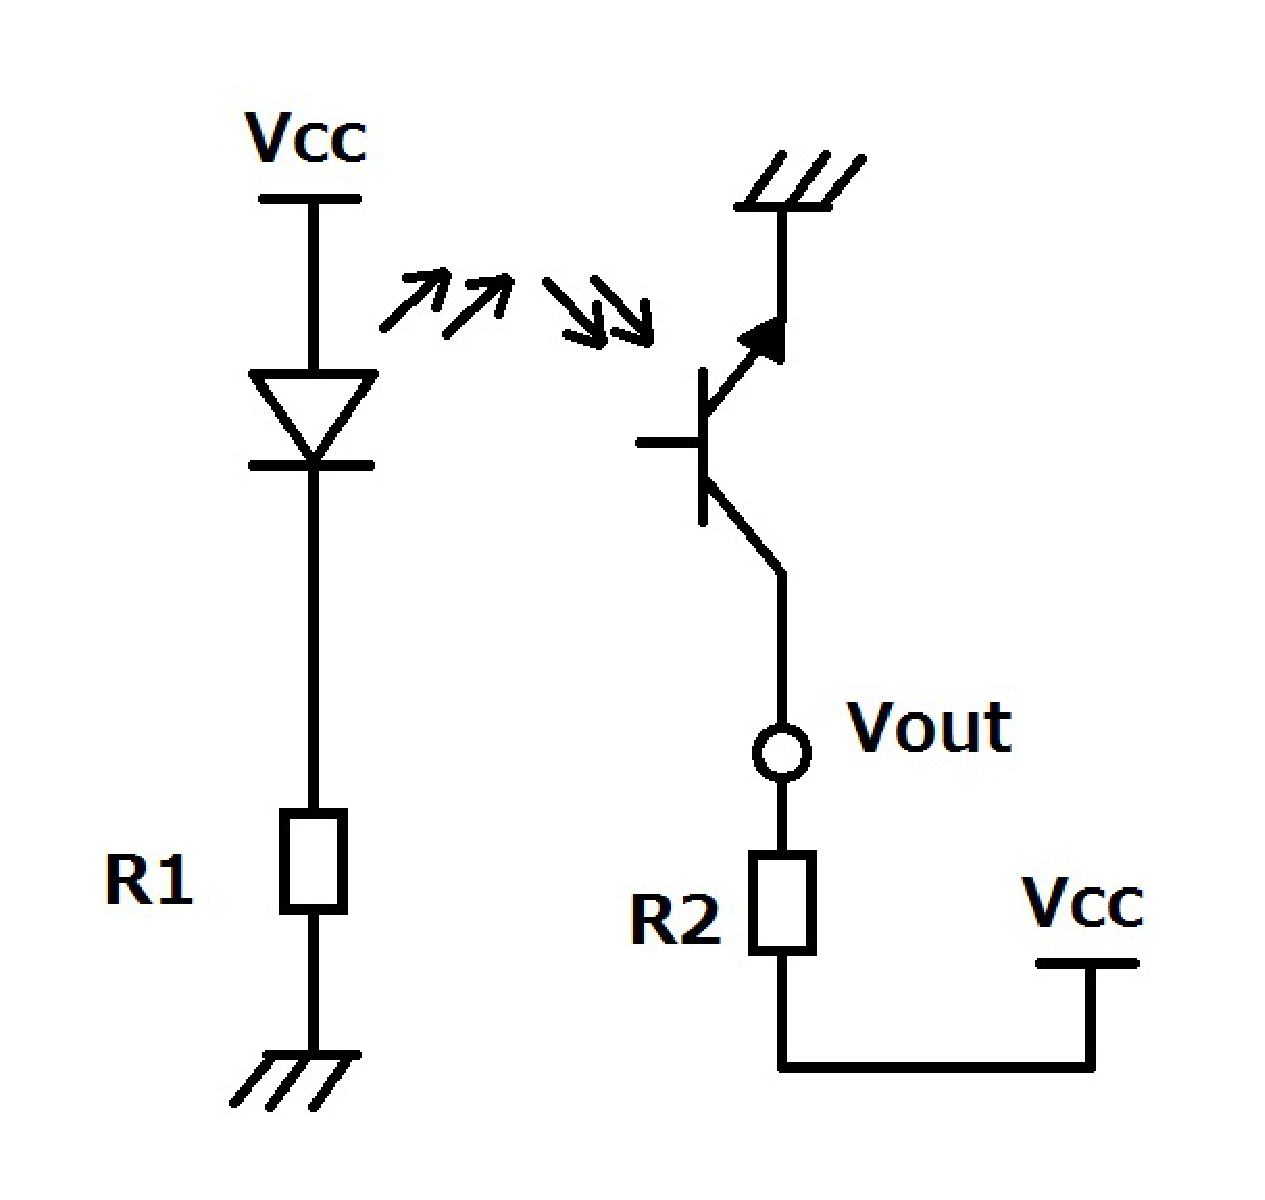
\includegraphics[width=0.2\linewidth]{Figs/tpr105_circuit}
		\caption{Photoreceptor circuit.}
		\label{fig:tpr105_circuit}
	\end{figure}
	The photoreceptors working principle is based on detecting the amount of reflected light. This controls the base current $i_B$ of the transistor in the schematic. This base current then determines the collector current $i_C$. Specific to this setup, the distance and therefore the output force controls the amount of light that is reflected on the wall of the palm pad. Therefore, we have:
	\begin{equation}
	F_{output} = k_{eq} \Delta x \propto i_B
	\end{equation}
	\begin{equation}
	i_C = h_{FE} i_B
	\end{equation}
	\begin{equation}
	V_{out} = V_{CC} - h_{FE} R_2 i_B = V_{CC} - K R_2 \Delta x
	\end{equation}
	Where $h_{FE}$ is the forward current gain and $K$ is a constant given by $h_{FE} k_{eq}$.
	
	The two resistor values have been empirically found to have the highest sensitivity but not saturating the measurement. The sensitivity decreases with a smaller resistor, since at a certain point, the Arduino cannot detect a change in voltage anymore. Saturation occurs, when the value of $R_2$ is too high.
	
	\subsection{Identification of Operational Range (Photoreceptor)}
	To find the receptor values at maximum compression of the springs, a simple test has been made, where one time $0$V has been applied to the motors, and another time $20$V has been applied. This $20$V value is within a safety margin of the maximum applicable voltage given by the datasheet of the motors. The result can be seen in figure \ref{fig:max_volt_applied_plot}.
	
	\begin{figure}[h!]
		\centering
		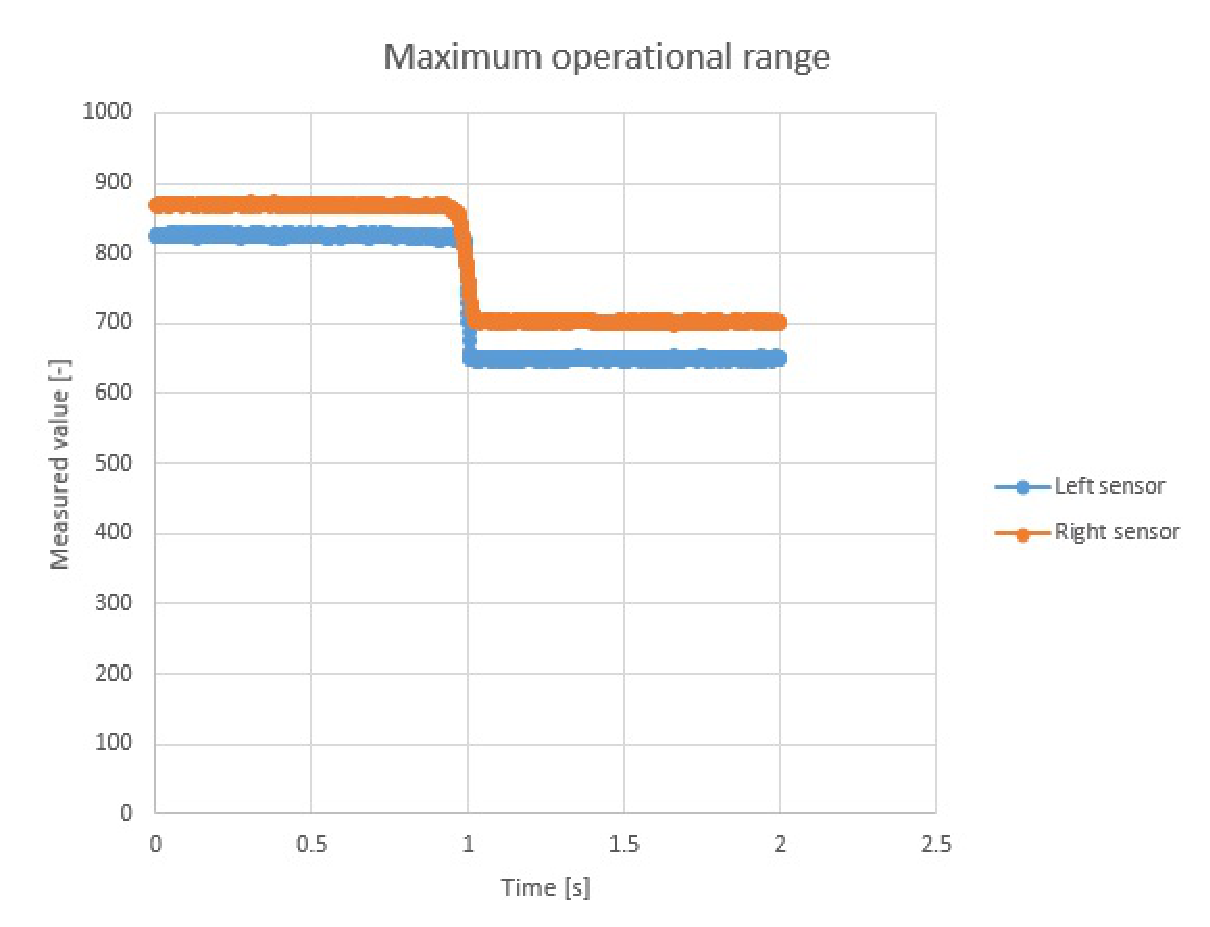
\includegraphics[width=0.6\linewidth]{Figs/max_volt_applied_plot}
		\caption{Operational range of photoreceptor with springs at rest and in full compression.}
		\label{fig:max_volt_applied_plot}
	\end{figure}
	
	The values that have been found to be the limiting values are resumed in table \ref{tab:oper_range_PS}.
	
	\begin{figure}[h!]
		\centering
		\begin{tabular}{|l|c|c|c|c|c|}
			\hline
			& Sensor reading & Distance & Sensor reading & Distance & Max output  \\
			& MAX (rest) & (rest) & MIN (compression) & (compression) & force \\ \hline \hline
			Left side & 830 & 2.35mm & 650 & 4mm & 9.9N \\ \hline
			Right side & 870 &2.2mm & 700 & 4mm & 10.8N \\ \hline
		\end{tabular}
		\caption{Identified operational range for the photoreceptors in the PlayStation controller.}
		\label{tab:oper_range_PS}
	\end{figure}
	
	Using these values, the photoreceptor measurements can be mapped to this range with an 8-bit value. This means that $0$ is no compression and $255$ is fully achievable compression.
	
	\section{Frequency Response Analysis}
	To conduct the frequency response analysis in a meaningful environment, the controller has to be tested under conditions close to the operational ones. To be able to control the distance between the palm pads and the L-plates, and therefore the compression ratio of the springs, the palm pads have been blocked mechanically. With the wave generator producing the reference signal, the Arduino controlled the motors to match the compression with the reference. Figures \ref{fig:1plot_zoom} to \ref{fig:100plot_zoom} show some testcases.
	
	
	\begin{figure}[!htb]
		\minipage{0.32\textwidth}
		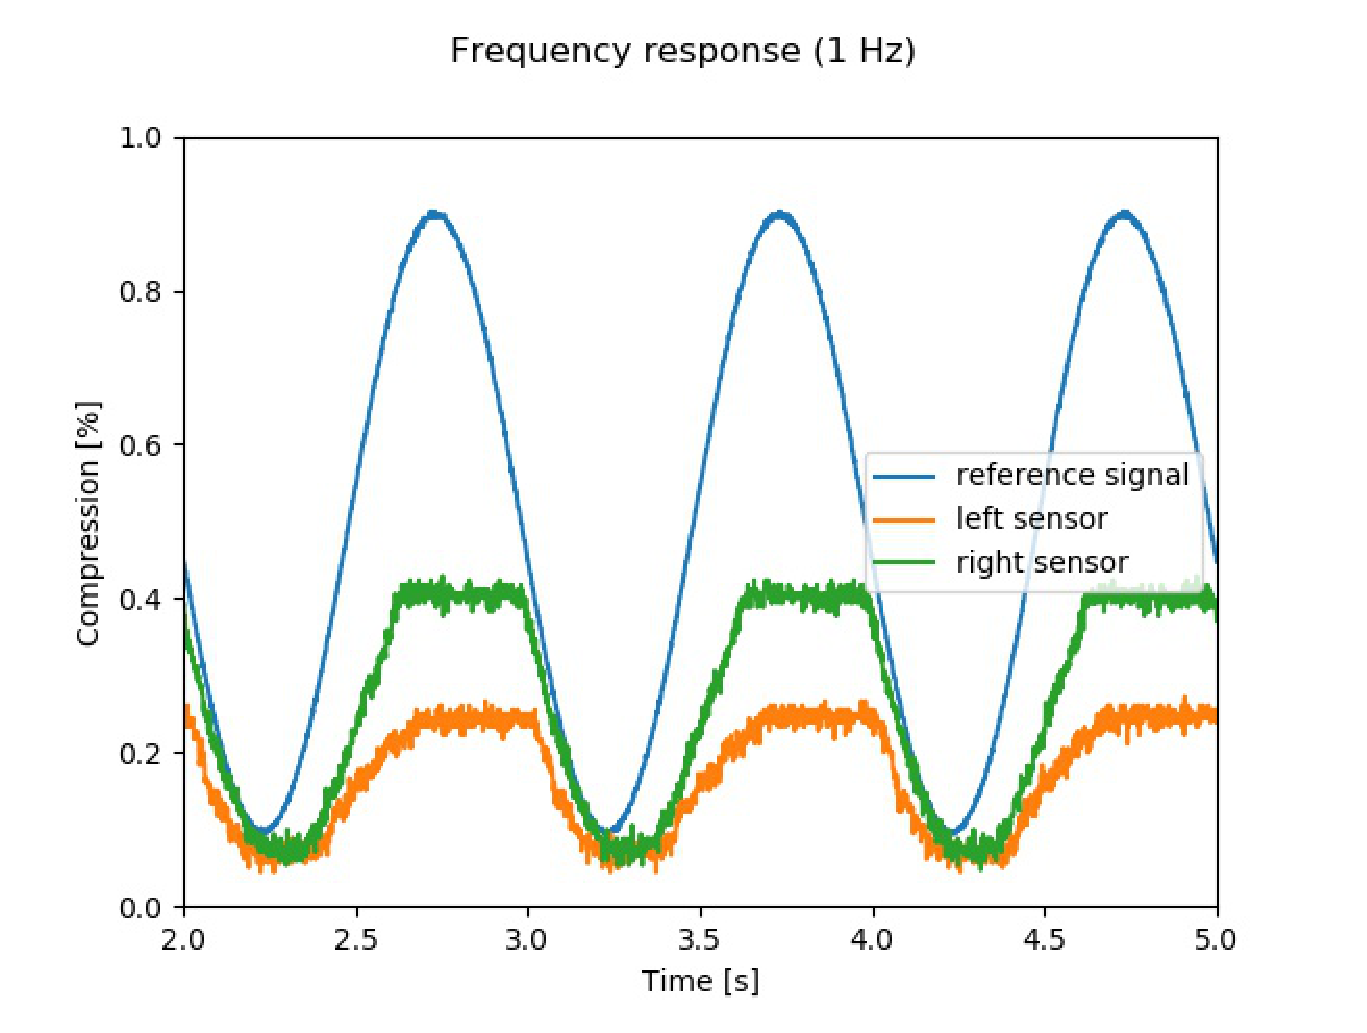
\includegraphics[width=\linewidth]{Figs/1plot_zoom}
		\caption{1 Hertz}\label{fig:1plot_zoom}
		\endminipage\hfill
		\minipage{0.32\textwidth}
		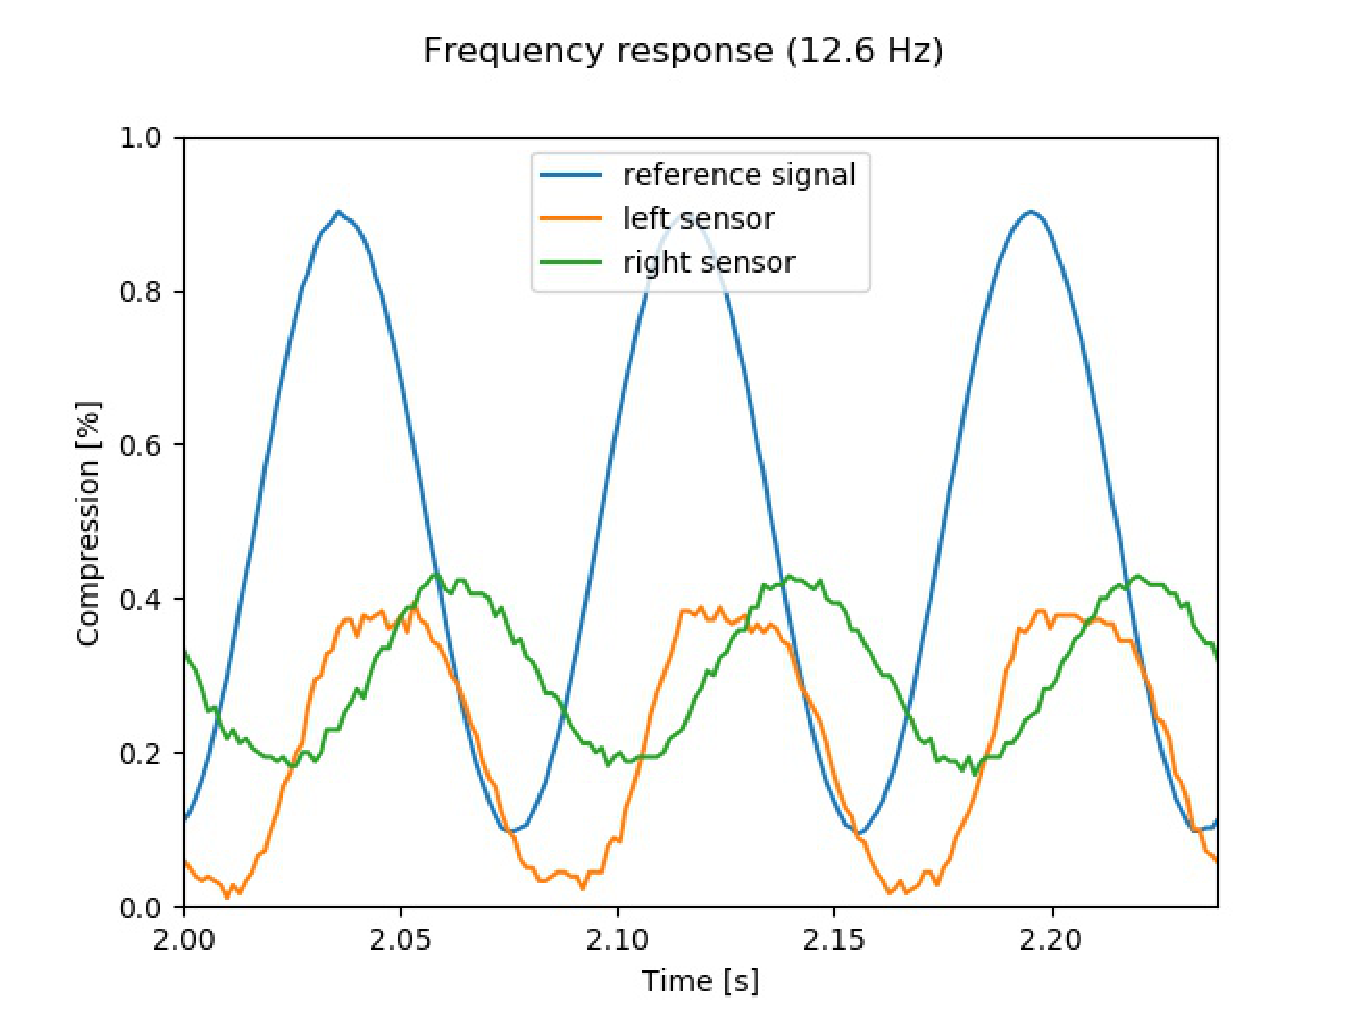
\includegraphics[width=\linewidth]{Figs/12.6plot_zoom.eps}
		\caption{12.6 Hertz}\label{fig:12.6plot_zoom}
		\endminipage\hfill
		\minipage{0.32\textwidth}%
		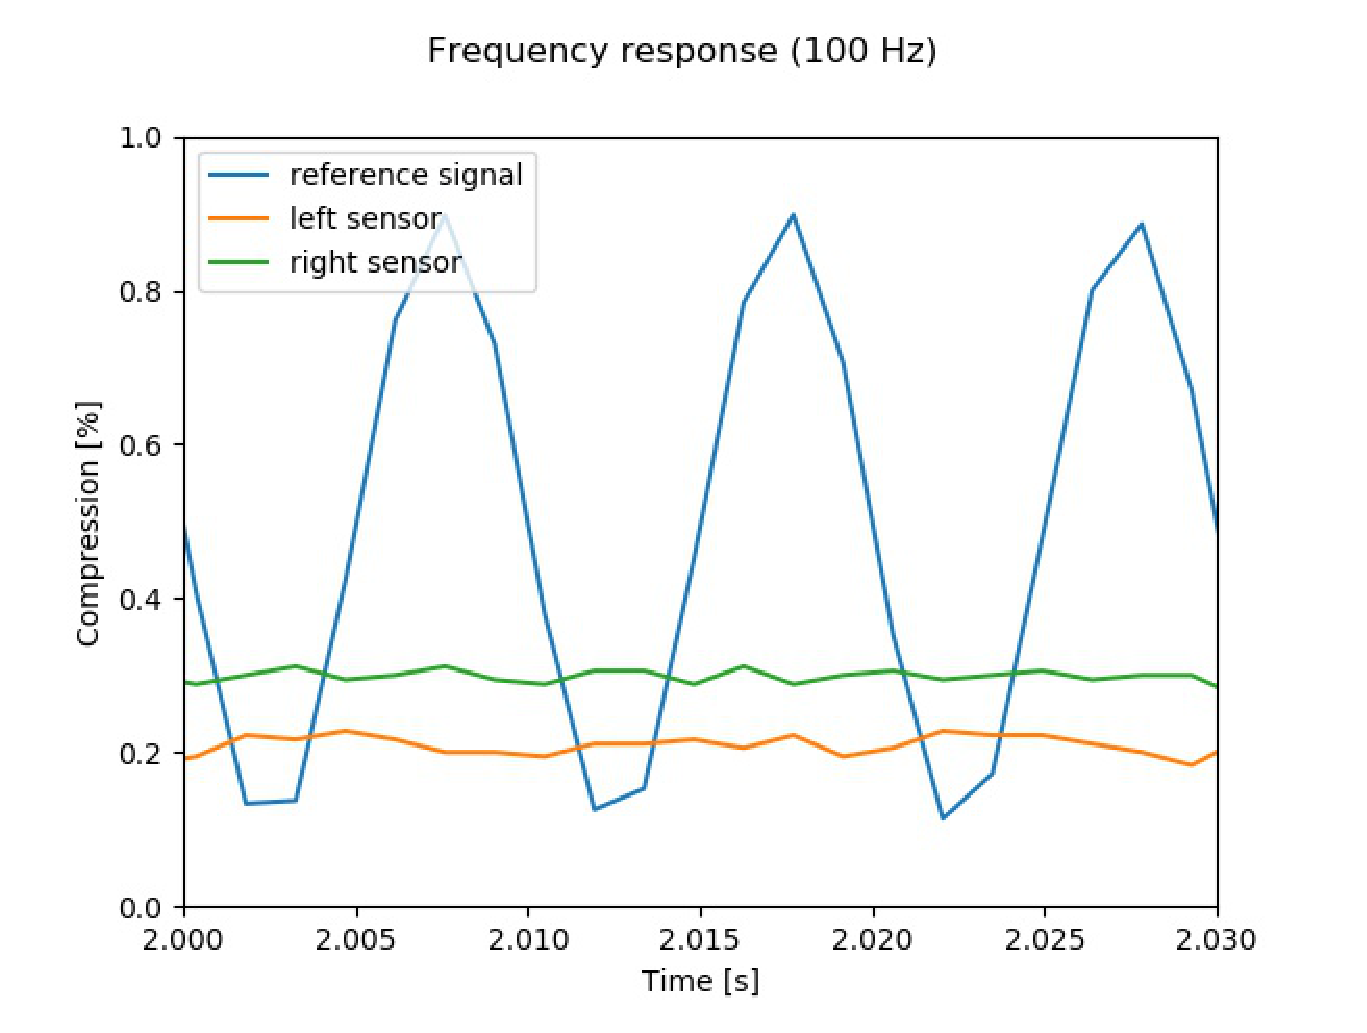
\includegraphics[width=\linewidth]{Figs/100plot_zoom}
		\caption{100 Hertz}\label{fig:100plot_zoom}
		\endminipage
	\end{figure}
	With these signals one can calculate the amplification factor between the reference signal and the output signal, as well as the phase shift.
	
	
	\subsection{Sinewave Fitting}
	As described in this example\cite{exnumerus2010}, one can fit a sinewave with the linear least square method to the samples. For finding the amplitude the second norm%TODO why not RMS as explained in slides_frf_and_bode_plots.pdf
	 has been used. This function returns the phase, amplitude and the bias. In this case, the difference in phase between input and output, as well as the amplitude ratio is needed in order to plot a Bode diagram.
	
	\subsection{Bode Diagram}
	The results of the frequency response analysis are shown in figures \ref{fig:bode_left} and \ref{fig:bode_right}.
	
	\begin{figure}[!htb]
		\minipage{0.48\textwidth}
		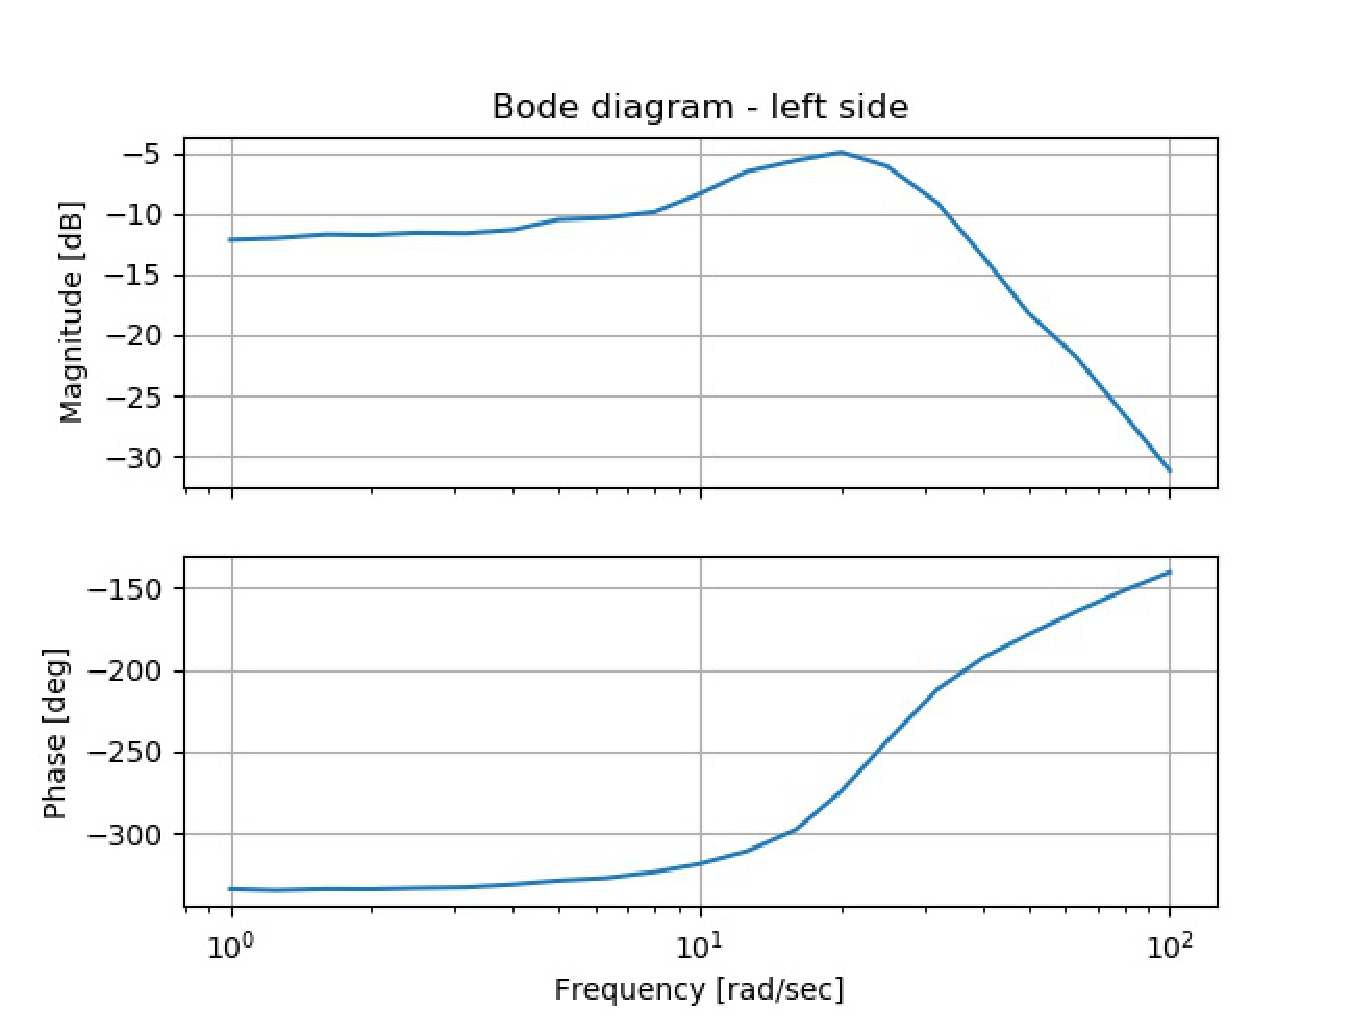
\includegraphics[width=\linewidth]{Figs/bode_left}
		\caption{Left-hand side, Motor reduction ratio $33:1$}\label{fig:bode_left}
		\endminipage\hfill
		\minipage{0.48\textwidth}
		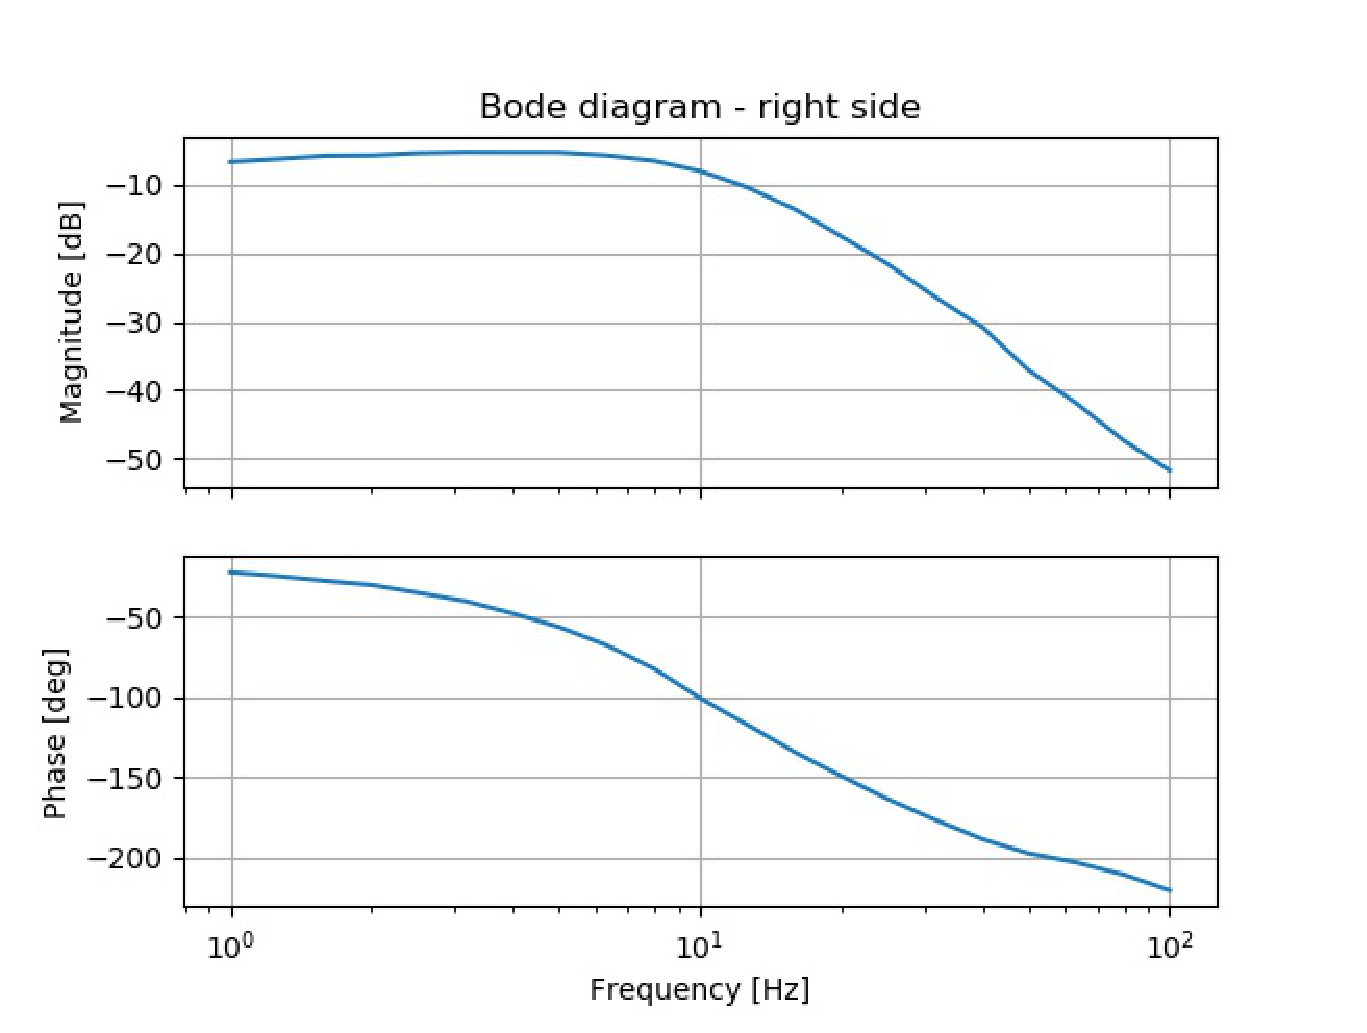
\includegraphics[width=\linewidth]{Figs/bode_right}
		\caption{Right-hand side, Motor reduction ratio $112:1$}\label{fig:bode_right}
		\endminipage\hfill
	\end{figure}

	For the left-hand side, a resonance top at around $13$Hz can be found, with a gain of roughly $-12$dB for lower frequencies. At higher frequencies a slope of roughly $-26$dB/dec has been calculated. For doing so the values in the range of $50$Hz and $100$Hz have been used. The phase shifts from $-25^\circ$ to $-222^\circ$, a total shift of roughly $200^\circ$.\\
	For the right-hand side, no resonance top is visible, and a constant gain of roughly $-6$dB for lower frequencies can be identified. At higher frequencies a slope of roughly $-30$dB/dec has been calculated. Again using the values in the range of $50$Hz and $100$Hz. The phase shifts from $-25^\circ$ to $-223^\circ$, a total shift of roughly $200^\circ$.
	%in slides_frf_and_bode_plots.pdf slide 27 suggests that the pole is stable since it goes from 0 to -180
	
	\section{Discussion}
	As it can be seen in figues \ref{fig:1plot_zoom} to \ref{fig:100plot_zoom} the signal is not followed very smoothly. For one, the magnitude ratio even at low frequencies is at roughly $0.5$. This shows that the proportional gain is too low. This would not only lift up the curve indicated in the Bode diagram and shift it towards higher frequencies (to the right). Another important aspect is the saturation behavior of the right motor. The origin of this effect  needs to be investigated in more detail.\\
	From the Bode diagrams one can conclude several things. First of all, the gain magnitude at lower frequencies should be around $0$dB to have perfect following of the reference signal. This can be influenced by tuning the proportional value of the controller.\\
	Second, the two motors show different characteristics. While the weaker motor (left-hand side) shows a resonance top around $13$ Herz, the stronger motor has no such behavior. In order to have a more linear system, it is therefore favorable to use the stronger motor for this spring system.\\
	Furthermore, the first pole of the system can be found around $13$ Herz. The communication frequency between robot and graphical user interface is suggested (according to the datasheet of the robot) to be between $1$Hz and $5$Hz. This shows that the series elastic actuator system as it is implemented in this experiment, is not the limiting factor in the robotic system.\\
	When one wants to determine the order of the system, one can look at the slope at the tail of the magnitude curve in the Bode plot. In our case they are $-26$dB/dec and $-30$dB/dec for left and right respectively. Since the slopes can only be a multiple of $20$dB/dec, it can be concluded, that the $2 \xi \omega _0$ term from equation \ref{eq:transfer_fn_2nd_order} has a non-negligible influence at the tail of the Bode plot.
	The equation of a second order transfer function is as follows:
	\begin{equation}
		H (s) = \frac{\omega _0^2}{s^2 + 2 \xi \omega _0 s + \omega _0^2}
		\label{eq:transfer_fn_2nd_order}
	\end{equation}
	Therefore one should also have a look at the phase lag diagram. The phase shift of roughly $180^\circ$ suggests a second order transfer function.
	
	The only thing that might risk the reliability of the Bode diagrams is the fact that the output signal has shown to be electrically interfering with the input signal. This most probably comes from the fact that the output impedance is too high.

	\section{Conclusion}
	The Bode diagrams show promising results. This is a first hint that the implementation of the series elastic actuators is not slowing down the system, since the bottleneck is given by the robot GUI communication link.\\
	
	\section{Outlook}
	The input signal is interfering with the output signal on the Arduino. Therefore it is necessary to investigate its impact by implementing a voltage follower to reduce the output impedance.\\
	A theoretical model shall be calculated to take into account the different aspects and parameters of the setup. The goal is to come up with a precise model to simulate different parameter settings, such as equivalent spring constant, motor parameters or operating frequency.
	

	
	%‚±‚±‚Ü‚Å
}










%+++++++++++++++++ June
	
	\section{Introduction}
	This report is the continuation of the first two reports about the project "Haptic Feedback Controller with Palm Pressurization". The last report has left off with the idea of implementing a voltage follower and suggested to retake measurements to create a Bode diagram. Furthermore, it has been suggested to create an analytical model and analysis of the setup in order to run simulations to identify setup parameters such as the equivalent spring constant, gain values or motor parameters.
	
	
	\section{Theoretical analysis}
	% I can check with existing papers and take their block diagram
	To come up with a theoretical analysis of the transfer function, a simplified mechanical schematic has been drawn. This schematic can be seen in figure \ref{fig:mechanical_schematic}.
	\begin{figure}[h!]
		\centering
		\includegraphics[width=0.6\linewidth]{Figs/mechanical_schematic}
		\caption{Simplified mechanical schematic of the actuation system with the stimulator.}
		\label{fig:mechanical_schematic}
	\end{figure}
	The equations of motion can be formulated with the major parameters defined in the schematic. A full explanation of all parameters can be seen in table \ref{tab:setup_params}. The variables with subscript $1$ refer to the first mass element, the carriage in its guideway, whereas variables with subscript $2$ refer to the stimulator, also known as the palm pad. For the motor the subscript $m$ has been used.
	
	\begin{figure}[h!]
		\centering
		\begin{tabular}{|l|c|c|}%designator | explanation | unit
			\hline
			 Designator & Explanation & Unit \\ \hline \hline
			$T_m$ & Motor torque & [Nm]\\ 
			$T$ & Output torque acting on carriage& [Nm]\\
			$\theta_m$ & Motor angle & [rad]\\
			$\theta$ & Clamp link angle & [rad]\\  
			$L_{CL}$ & Clamp link length & [m]\\
			$m_{1}$ & Mass of the carriage in its guideway & [kg]\\
			$m_{2}$ & Mass of the stimulator & [kg]\\
			$x_{1}$ & Position of the carriage in its guideway & [m]\\
			$x_{2}$ & Position of the stimulator & [m]\\
			$k_{eq}$ & Equivalent spring constant & [N/m]\\
			$b_{sp}$ & Spring damping coefficient & [Ns/m]\\
			$n$ & Reduction gear ratio & [-]\\
			$k_{op}$ & Spring constant of the operator & [N/m]\\
			$b_{op}$ & Damping coefficient of the operator & [Ns/m]\\
			$J_T$ & Total inertia of mechanical setup & [$\textit{kgm}^2$]\\
			\hline
		\end{tabular}
		\caption{Setup parameters}
		\label{tab:setup_params}
	\end{figure}
	
	\subsection{Assumptions}
	First of all, it is important to mention that the transfer function is non-linear, due to the motor angle $\theta_m$ that determines the force acting on the carriage with mass $m_1$. As an initial approach however, this effect has been neglected. More specifically, it is assumed that $\theta \ll 1$ and $\cos{(\theta)} \frac{T_m}{L_{CL} } = F_{carr} $ becomes $\frac{T_m}{L_{CL} } \simeq F_{carr} $. Here the angle $\theta$ is the angle of the lever, pushing the carriage (ie. $\theta_m = n \theta$). \\
	Furthermore, there are several types of friction in the system: the intrinsic friction within the motor and its reduction gear, inside the bearings and the carriage in its guideway. Additionally the springs have a non-negligible damping coefficient. In this work the overall friction and the spring damping have been merged and are represented by the friction coefficient $b_{sp}$. The stimulator, is not in contact with the controller, but with the operator. To model the damping of the skin of the operator and the friction between the skin and the palm pad, the damping coefficient $b_{op}$ has been introduced. Similarly the spring constant of the operator's skin is modeled by $k_{op}$.\\
	
	\subsection{Spring Constant and Damping Coefficient of the Operator's Hands}
	The order of magnitude of the two coefficients $k_{op}$ and $b_{op}$ are discussed in \cite{Kuchenbecker2003} \cite{Park2014} \cite{Speich2005}. They all indicate parameters varying in the same order of magnitude, namely $k_{op} \simeq 400$N/m and $b_{op} \simeq 5$Ns/m.\\
	
	\subsection{Identification of the Spring Damping Coefficient}
	The damping coefficient of the spring $b_{sp}$ can be found by comparing the theoretical results of the frequency response analysis with the experimental findings. In fact, for the experimental setup, the stimulator has been fully blocked and therefore the operator's spring coefficient can be seen as infinitely stiff.\\
	By varying $b_{sp}$ and Bode-plotting the results of the analytical transfer function, the coefficient's order of magnitude can be found. In order to do so, the analytical transfer function has to be identified.
	
	\subsection{Expected Transfer Functions}
	The system can be cut into two major transfer functions. The block diagram including these two transfer functions is depicted in figure \ref{fig:2tf_block_diagram}. 
	
	\begin{figure}[h!]
		\centering
		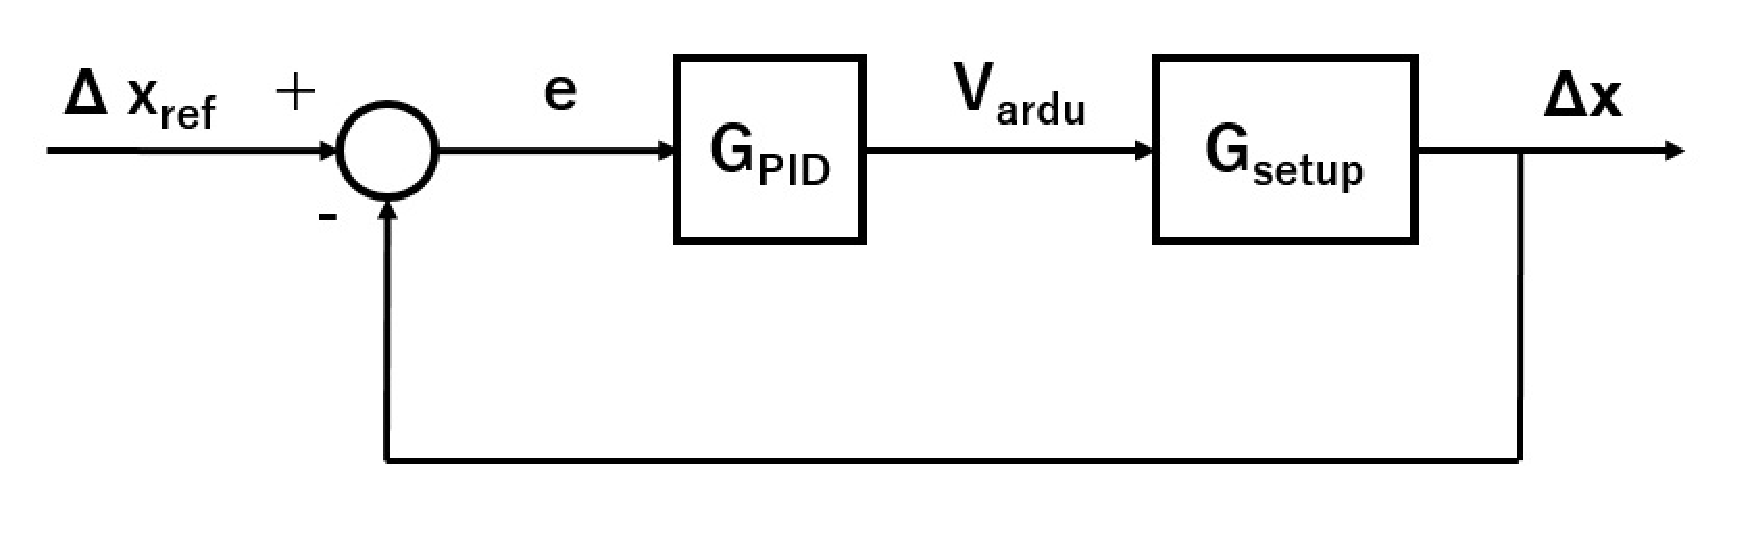
\includegraphics[width=0.6\linewidth]{Figs/2tf_block_diagram}
		\caption{Block diagram with two different transfer functions.}
		\label{fig:2tf_block_diagram}
	\end{figure}
	According to this figure one can obtain a transfer function of the following form:
	\begin{equation}
		F(s) = G_{PID}(s)G_{setup}(s) = \frac{V_{ardu}}{E}\frac{\Delta X}{V_{ardu}} = \frac{\Delta X(s)}{E(s)}
		\label{eq:complete_tf}
	\end{equation}
	where $V_{ardu}$ is the voltage output of the arduino for controlling the motors. Using this form one can calculate the individual transfer functions and finally relate the compression of the springs $\Delta x$ to the compression given as reference $\Delta x_{ref}$, since $\Delta X_{ref} / \Delta x = F/(1+F)$.
	
	\subsubsection{PID Transfer Function}
	The transfer function given by the PID-controller is very straight-forward and can be taken out of any control theory book \cite{Dutton1997}. 
	Since the arduino has limited resolution with floating point operations, the error and reference has been converted into micrometers. To keep the gains consistent between the arduino code and the matlab script for analytical analysis, the multiplication factor $K_{\mu m}$ to get from the reference distance in meters to micrometers has been introduced. Furthermore, an offset has been added ($K_{bit-offset} = 128$) to allow for negative armature voltages and lastly the PID value has been converted to the arduino output voltage, where $255$ corresponds to $5$ V. The transfer function is given in equation \ref{eq:tf_pid}. 
	\begin{equation}
		G_{PID} (s) = \frac{V_{ardu}(s)}{E(s)} = (K_{\mu m} (K_P + \frac{K_I}{s} + K_Ds) +K_{bit-offset}) K_{PID2Vardu}
		\label{eq:tf_pid}
	\end{equation}
	Finally, there is also the gain of the amplifier in voltage mode, which converts the voltage of the arduino into the voltage applied to the motors. This gain is $K_{ampl} = 10$Volt/Volt. To this voltage an offset voltage of $V_{offset} = -25$V is added.\\
	
	\subsubsection{Motor Equations}
	The second transfer function relates the motor torque $T_m$ to the arduino voltage as well as the output $\Delta x$ to $T_m$. Due to the back electromotive force these two parts are related and have to be treated as a whole.
	
	The output torque $T_m$ of the motor can be calculated using the sum of all torques and the conversion parameters intrinsic to the motor.\\
	Similar to the setup and analysis in \cite{Junior2016} the equations of the motor are given as:
	\begin{equation}
		L_a \frac{di_a}{dt} + R_a i_a + K_{emf} \dot{\theta }_m = V_a
	\end{equation}
	where $L_a$ is the armature inductance, $R_a$ the armature resistance and $i_a$ the armature current of the motor. $K_{emf}$ is the back electromotive force constant also given by the motor. $V_a$ is the armature voltage and $\theta_m$ is the angle of the motor shaft.\\
	Furthermore, with Newton's law, the sum of all torques must be zero, or:
	\begin{equation}
		J_{T} \ddot{\theta }_m - \frac{k_{eq} L_{CL}}{n} \Delta x - \frac{b_{sp} L_{CL}}{n} (\dot{x}_2 - \dot{x}_1)  = T_m = K_{\tau} i_a
		\label{eq:torques}
	\end{equation}
	In equation \ref{eq:torques} the parameter $J_{T}$ stands for the total equivalent inertia of the motor, the clamping link and the carriage of mass $m_1$.  $K_{\tau}$ is the proportional current torque gain constant. The moment of inertia can either be calculated as the sum of all inertias seen by the motor shaft, or measured in a simple test.\\ 
	
	\subsection{Analytical Inertia Identification}
	The total inertia of the system is determined by the inertia of the rotor and gears $J_m$, the inertia of the clamp link $J_{CL}$ as well as the inertia of the carriage assembly with mass $m_1$. The last one can be found by simplifying the load to a point mass at distance of the clamp link's length $L_{CL}$, which yields a moment of inertia of $J_{carr} = m_1 L_{CL}^2$.
	The gear box affects the inertia seen by the motor shaft by the square of its ratio $n$:
	\begin{equation}
		J_{reflected} = \frac{ J_{load}}{n^2}
	\end{equation}

	We therefore have a total inertia of:
	\begin{equation}
		J_T = J_m + \frac{J_{CL}}{n^2} + \frac{ m_1 L_{CL}^2}{n^2}
	\end{equation}
	where $J_{CL}$ can be calculated by approximating it as a cantilever with an off-center axis of distance $L_{CL} /2$ \footnote{(2018, June 19th) retrieved from \url{http://www.orientalmotor.com/technology/motor-sizing-calculations.html}}: %Source: http://www.orientalmotor.com/technology/motor-sizing-calculations.html
	
	\begin{equation}
		J_{CL} = \frac{1}{12}m_{CL}(A^2 + B^2 + 12l^2)
	\end{equation}
	where $A$ and $B$ are the width and length respectively.\\
	The calculated total moment of inertia for the motor with a reduction ration of $n = 112$ is $J_T = 6.87 \times 10^{-8}$ $\textit{kgm}^2$.
	
	\subsection{Experimental Inertia Identification}
	Alternatively, one can approximate the total moment of inertia by applying a constant current on the motor and measuring the acceleration. In this case the traveled distance has been derivated twice to find the acceleration, which results in an amplification of errors. Furthermore, the constant current has been kept very low, (between $20$ and $100$ mA), which led to a slow movement and therefore higher friction impact on the measurements. However, the results are consistent with the theoretically calculated values:
	$$ J_T = \frac{7.5 \times 10^{-4}}{n^2} = 5.98 \times 10^{-8} \textit{ kgm}^2$$ 
	
	\subsection{Relating $\Delta X$ to $\theta$}
	The conversion between the angle $\theta$ and the carriage's traveled distance $x_1$ can be found by assuming that the horizontal displacement of the carriage is given by $L_{CL} sin(\theta) = x_1$. For small angles of $\theta$ the Taylor expansion gives:
	\begin{equation}
		L_{CL} \theta \simeq x_1
		\label{eq:assum}
	\end{equation} 
	
	The output $\Delta x$ is the compression of the springs and is given by $\Delta x = x_2 - x_1$. For finding $x_2$ the equation of motion given by Newton's law has been considered.
	
	\begin{equation}
		m_2 \ddot{x}_2 = -k_{eq} (x_2 - x_1) - b_{sp} (\dot{x}_2 - \dot{x}_1) - k_{op} x_2 - b_{op} \dot{x}_2
		\label{eq:mov_stimul}
	\end{equation}
	In the case where the stimulator has been blocked by a wall, $\dot{x}_2$ has been forced to zero. Using the Laplace transform and equation \ref{eq:mov_stimul} one finds the expression of $x_2$:
	
	\begin{equation}
		X_2 = -\frac{k_{eq} + b_{sp} s}{s^2 m_2 + b_{op} s + k_{op}} \Delta X
		\label{eq:x2dx}
	\end{equation}
	
	\subsubsection{Motor and Spring Transfer Function}
	Combining all the equations one can find the final block diagram, which can be seen in figure \ref{fig:block_diagram}
	\begin{figure}[h!]
		\centering
		\includegraphics[width=0.95\linewidth]{Figs/block_diagram}
		\caption{Complete block diagram relating the output $\Delta x$ to the input $\Delta x_{ref}$.}
		\label{fig:block_diagram}
	\end{figure}


	From this diagram and the equations mentioned above, one can obtain the transfer functions that relate the output $\Delta x$ and input $\Delta x_{ref}$ as introduced in equation \ref{eq:complete_tf},
	where $\Delta X(s)$ and $\Delta X_{ref}(s)$ are the Laplace transforms of the output and input functions respectively. \\
	It is thus possible to study the frequency response by simulating this setup with the assumptions mentioned earlier.
	
	\subsection{Main Equations for Analytical Transfer Function}
	\begin{equation}
		\Delta X_{ref} - \Delta X = E
		\label{eq:error}
	\end{equation}
	
	\begin{equation}
		((K_P + K_D s + \frac{K_I}{s})E K_{\mu m} + K_{bit-offset}) K_{PID2Vardu} K_{ampl} + V_{offset}= V_a
		\label{eq:PID}
	\end{equation}
	
	\begin{equation}
		\frac{V_a - K_{emf}\dot{\theta}_m}{L_a s + R_a} K_{\tau} + F_{coupled} = J_T \ddot{\theta}_m
		\label{eq:motor_torques}
	\end{equation}
	
	\begin{equation}
		F_{coupled} = (k_{eq} + b_{sp}s) \frac{L_{CL}}{n} \Delta X
		\label{eq:fcoupled}
	\end{equation}
	
	\begin{equation}
		\theta_m = \frac{n}{L_{CL}} X_1 = -\frac{n}{L_{CL}}(1 + \frac{k_{eq} + b_{sp}s}{m_2 s^2 + b_{op}s + k_{op}}) \Delta X
	\label{eq:theta}
	\end{equation}
	
	Note that the constant offsets in equation \ref{eq:PID} are for pure symmetrical reasons and will cancel each other out, since $K_{bit-offset} K_{PID2Vardu} K_{ampl} + V_{offset} = 0$ and the equation becomes $ ((K_P + K_D s + \frac{K_I}{s})E K_{\mu m} ) K_{PID2Vardu} K_{ampl}= V_a$. This is the equivalent to a standard PID form with gains $K'_P$, $K'_D$ and $K'_I$.\\
	In the case of the experimental setup the palm pad has been blocked and therefore $x_2$ has been forced to be constant. The last equation becomes thus: $\theta_m = - \frac{n}{L_{CL}} \Delta X$.
	
	\subsection{Tracking Behavior of the P-controller}
	The tracking behavior of the P-controlled setup can be seen in the following figures.
	\begin{figure}[h!]
		\centering
		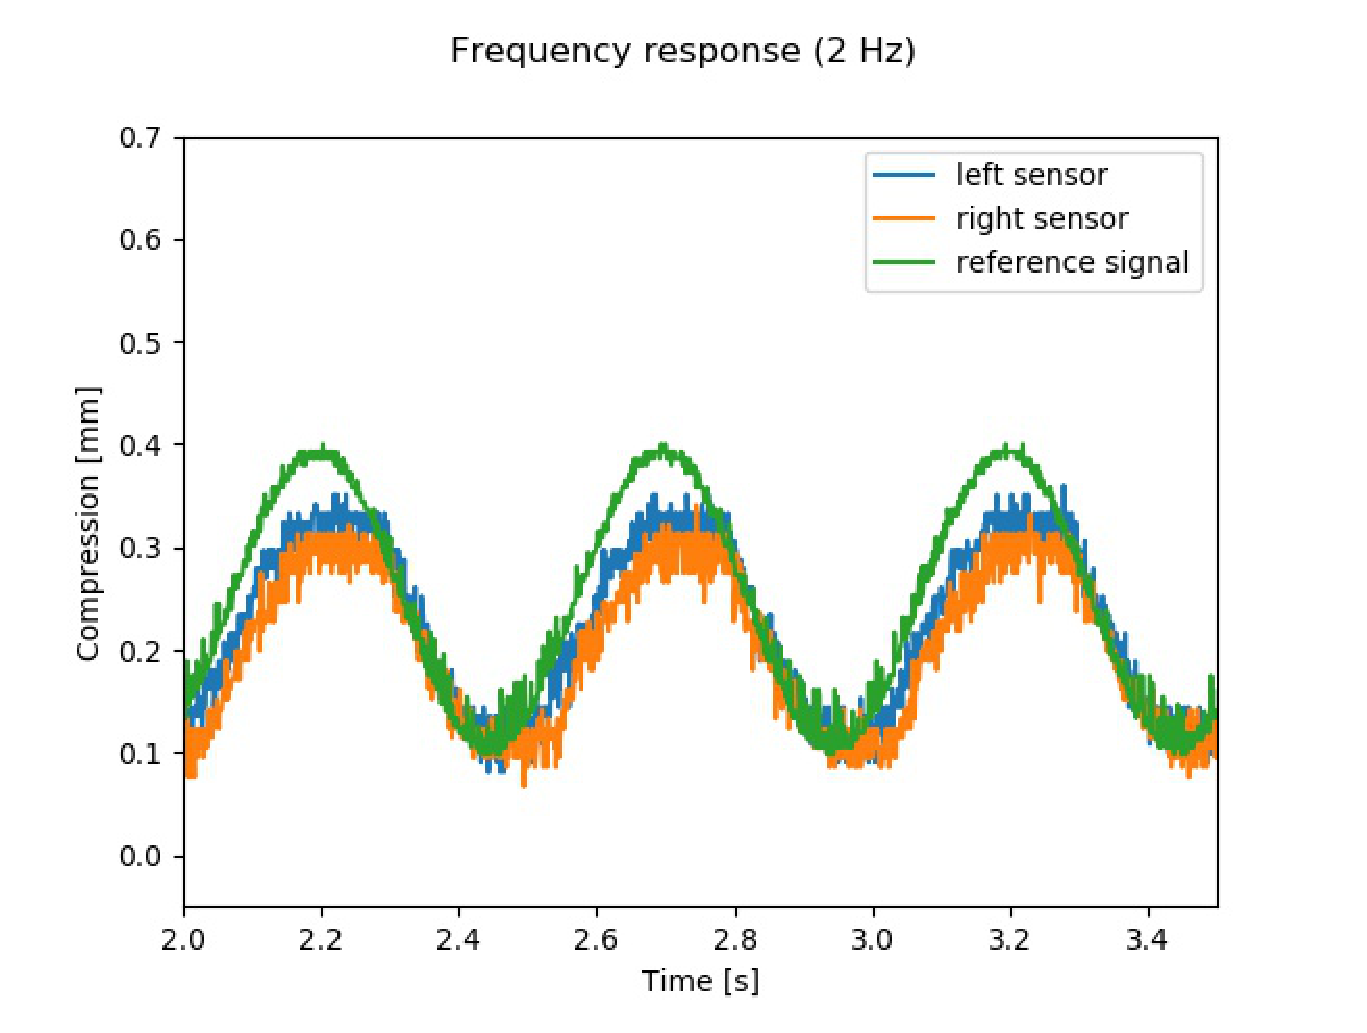
\includegraphics[width=0.6\linewidth]{Figs/2plot_zoom_P}
		\caption{Tracking behavior of the P-controller for $2$ Hz.}
		\label{fig:2plot_zoom_P}
	\end{figure}
	\begin{figure}[h!]
		\centering
		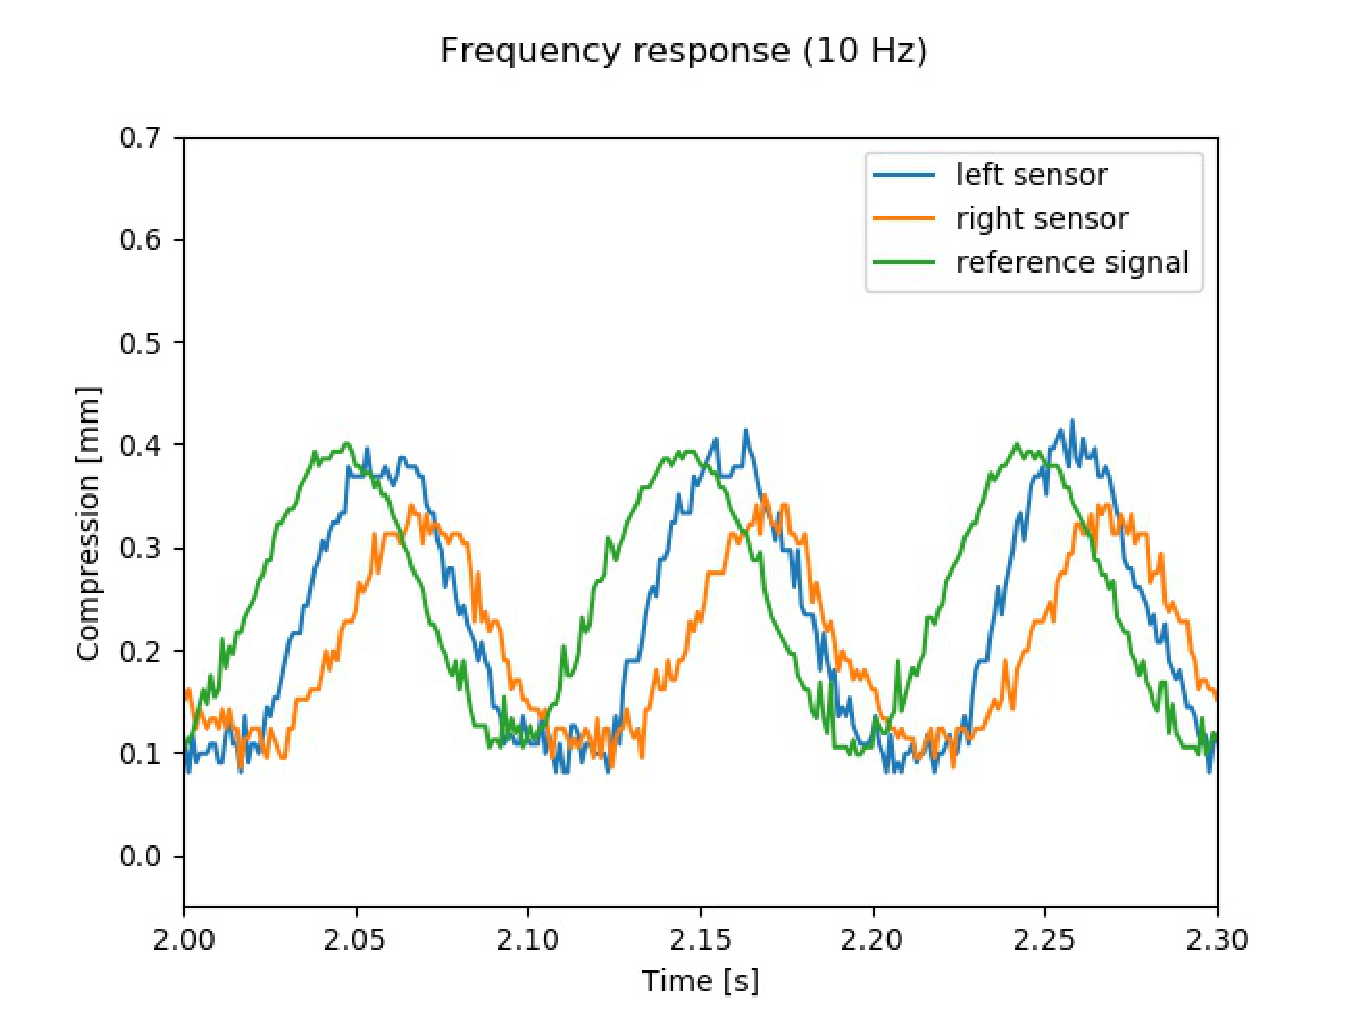
\includegraphics[width=0.6\linewidth]{Figs/10plot_zoom_P}
		\caption{Tracking behavior of the P-controller for $10$ Hz.}
		\label{fig:10plot_zoom_P}
	\end{figure}
	
	%show picture, explain problem of steady state offset, find PID values
	
	\subsection{Comparison of Results - P-controller and Experimental Data}
	The analytical transfer function has only been calculated for a specific set of spring damping coefficients $b_{sp}$. The results for the uniformly spaced values between $100$Ns/m and $400$Ns/m are depicted in figure \ref{fig:bode_all_combined_P02}. The gains that have been used are for a P-controller, it was namely $K_P' = 39.2 \frac{\textit{V}}{\textit{mm}}$. The simulation result that was closest to the experimental setup can be seen in figure \ref{fig:bode_sp_damp300_P02} and the corresponding transfer function is:
	\begin{equation}
		%\frac{\Delta X}{\Delta X_{ref}} = \frac{7.04\times 10^{-3} s^2 + 288 s + 2.94\times 10^{6}}{1.09\times 10^{-10}s^5 + 6.69\times 10^{-6}s^4 + 0.137 s^3 + 940s^2 +6.45 s + 2.95\times 10^{6}}
		\frac{\Delta X}{\Delta X_{ref}} = \frac{1.23 \times 10^3}{3.24\times 10^{-6}s^3 + 6.67\times 10^{-2}s^2 + 8.48s + 1.23 \times 10^3}
	\end{equation}
	

\begin{figure}[h!]
	\centering
	\includegraphics[width=0.6\linewidth]{Figs/bode_all_combined_P02}
	\caption{Bode plot comparison of experimental data of the P-controller and analytical transfer functions for several different $b_{sp}$.}
	\label{fig:bode_all_combined_P02}
\end{figure}

\begin{figure}[h!]
	\centering
	\includegraphics[width=0.6\linewidth]{Figs/bode_sp_damp300_P02}
	\caption{Bode plot comparison of experimental data of the P-controller and analytical transfer function for $b_{sp} = 300$Ns/m.}
	\label{fig:bode_sp_damp300_P02}
\end{figure}

%	\begin{figure}[h!]
%		\centering
%		\begin{subfigure}{.5\textwidth}
%			\centering
%			\includegraphics[width=0.6\linewidth]{Figs/bode_all_combined_P02}
%			\caption{Bode plot comparison of experimental data of P-controller and analytical transfer functions for several different $b_{sp}$.}
%			\label{fig:bode_all_combined_P02}
%		\end{subfigure}%
%		\begin{subfigure}{.5\textwidth}
%			\includegraphics[width=0.6\linewidth]{Figs/bode_sp_damp300_P02}
%			\caption{Bode plot comparison of experimental data of P-controller and analytical transfer function for $b_{sp} = 300$Ns/m.}
%			\label{fig:bode_sp_damp300_P02}
%		\end{subfigure}
%		%\caption{A figure with two subfigures}
%		%\label{fig:test}
%	\end{figure}



As it can be seen in figure \ref{fig:bode_sp_damp300_P02} there is a constant gain of $1$ for lower frequencies and a slight resonance top becomes visible around $18$Hz. The phase shift is of around $-210^\circ$ for the tested frequencies, and the lag does not increase more than $45 ^\circ$ for the frequencies of interest. Due to the setup constraints, the analytical results of higher frequencies have not been considered.

\subsection{Motor Comparison}
When one goes back to the experimental results where the two motors with different reduction gear ratios have been compared (previous report), %TODO make reference here, put up to date photos
one can conclude that the motor with the higher reduction ratio has a higher output force with a tradeoff of speed. Since one of the critical elements of the SEA system is its actuation speed, it is essential to push the boundaries as far as possible. However, the high gain frequency response in the experimental setup starts to drop at much higher frequencies than the actual operating frequency (which is given by the rather slow communication speed between the robot and the control device of $f_{op} \simeq 2-5$ Hz).\\
Due to the fact that even with the stronger reduction gear motor, the springs cannot be compressed to their limits, a higher possible output force has been favored and therefore the stronger motor seems more appropriate.

\subsection{Experimental PID Tuning}
At first, the Ziegler Nichols tuning method has been used to identify the PID gains for the setup. However, due to the non-linear behaviour, these gains resulted in a rather poor tracking performance of the reference signal.\\
Since an educated tuning of the gains is the very core problem of all control engineering, a lot of different approaches exist to find optimal or sub-optimal gain values. Given the complexity of the setup, it seemed reasonable to go for the simple trial and error approach, where the gains have been tuned and the tracking performance was shown in real-time. This approach led to the following gain coefficients:

%TODO discuss the fact of neglected efficiency, what is backdriveability exactly, redo bode plot with new pid settings 
\begin{figure}[h!]
	\centering
	\begin{tabular}{|l|c|c|}
		\hline
		Designator & Value & Unit \\ \hline \hline
		$K'_P$ & $47.6$ & [V/mm]\\ 
		$K'_I$ & $0.124$ & [V/mm/s]\\
		$K'_D$ & $247$ & [Vs/mm]\\
		\hline
	\end{tabular}
	\caption{Trial and error PID tuning.}
	\label{tab:trial_error_pid}
\end{figure}


\subsection{Tracking Behavior of the PID-controller}
The tracking behavior of the P-controlled setup can be seen in the following figures.
%show picture, explain problem of steady state offset, find PID values
\begin{figure}[h!]
	\centering
	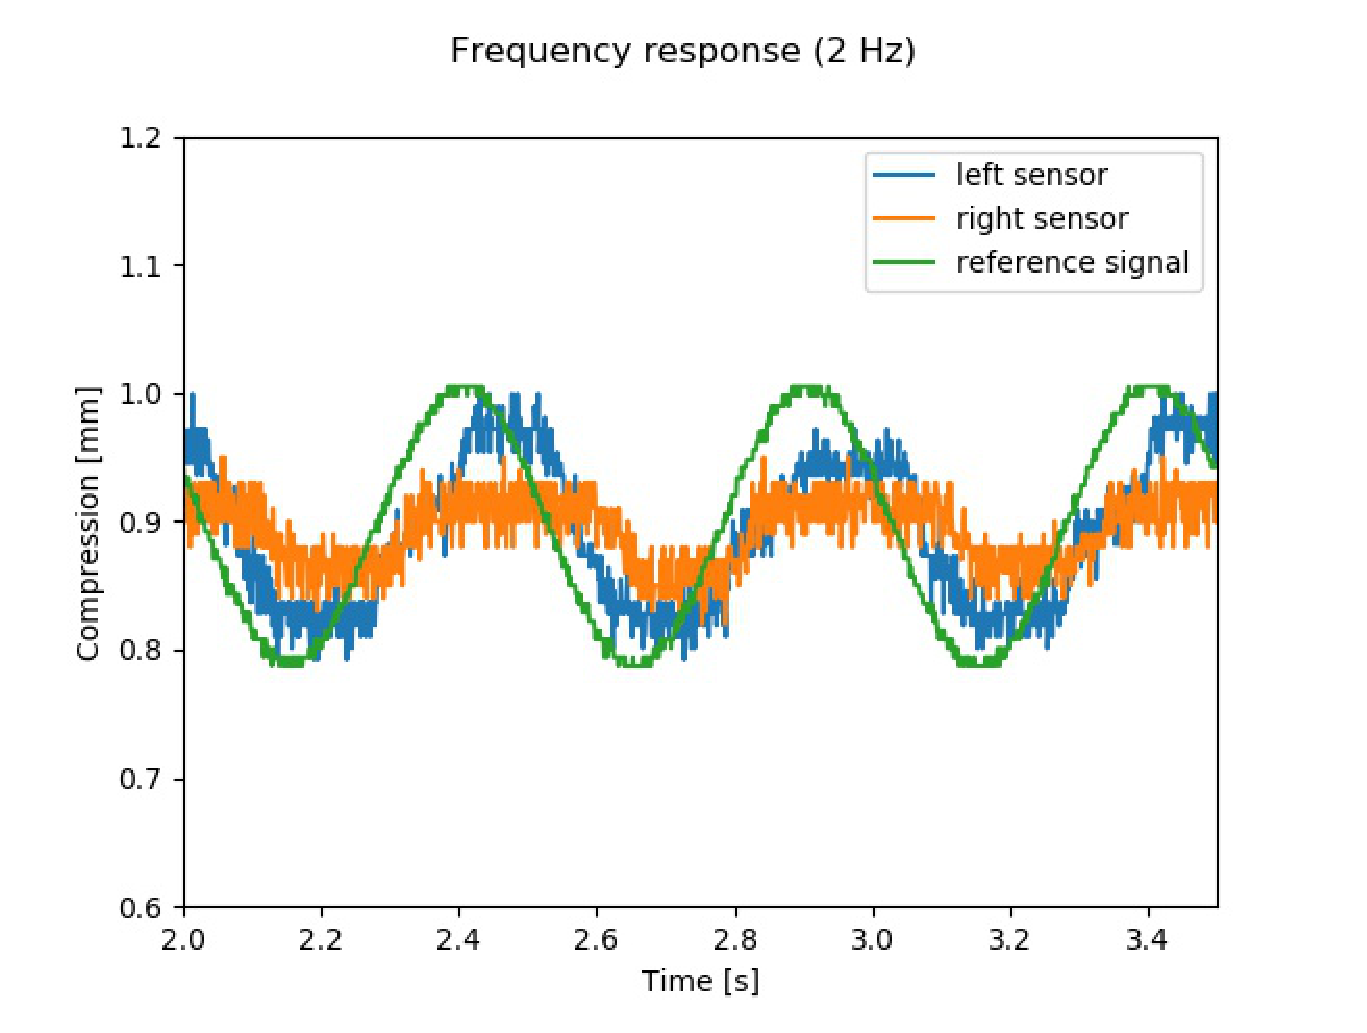
\includegraphics[width=0.6\linewidth]{Figs/2plot_zoom_PID}
	\caption{Tracking behavior of the PID-controller for $2$ Hz.}
	\label{fig:2plot_zoom_PID}
\end{figure}
\begin{figure}[h!]
	\centering
	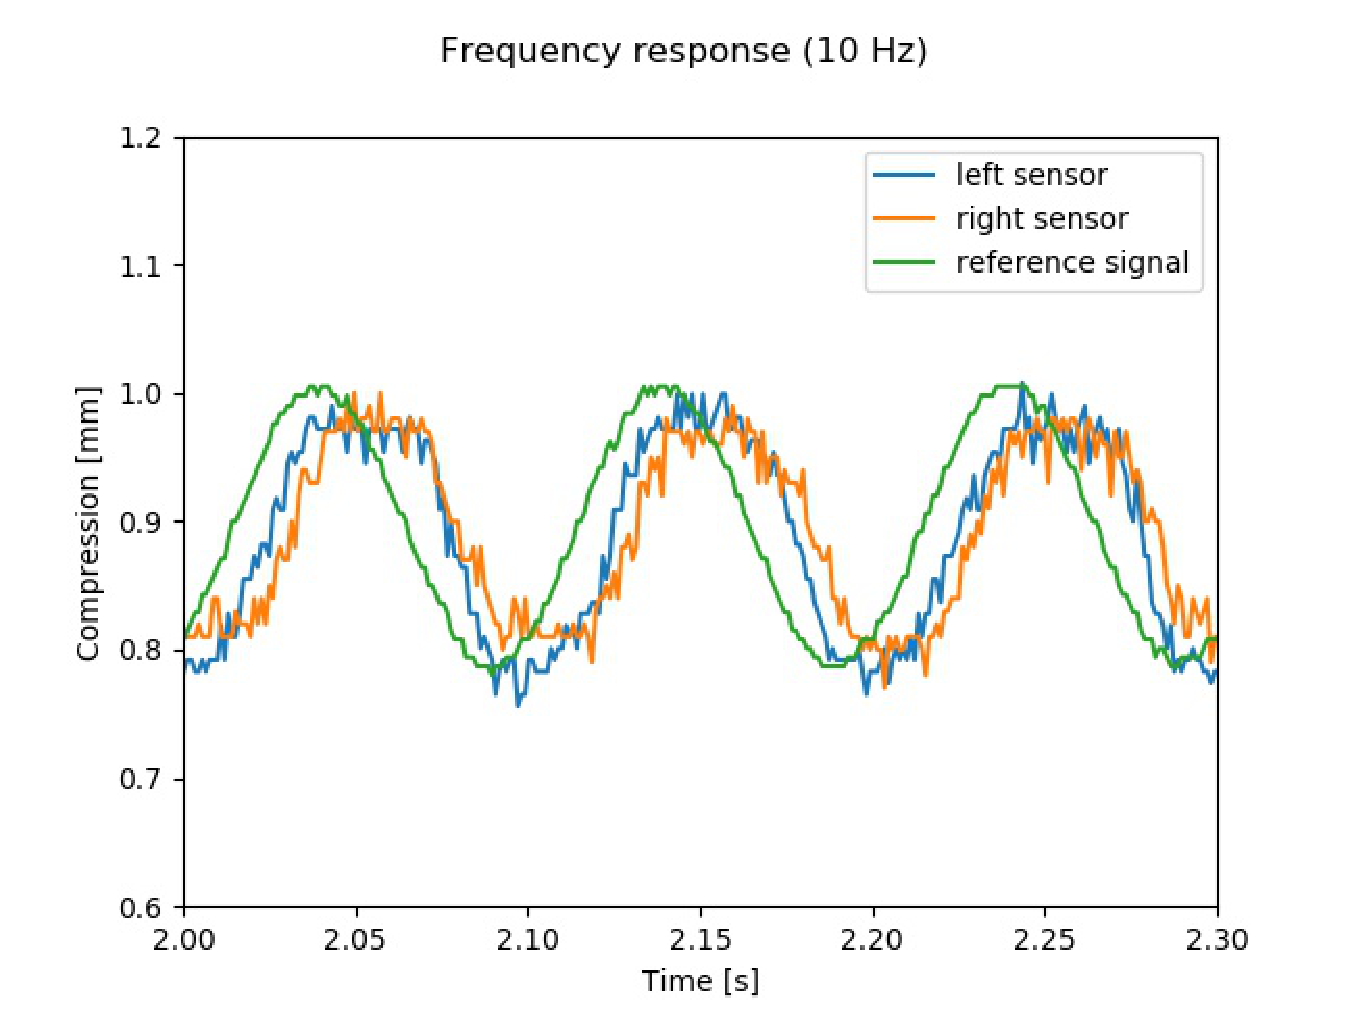
\includegraphics[width=0.6\linewidth]{Figs/10plot_zoom_PID}
	\caption{Tracking behavior of the PID-controller for $10$ Hz.}
	\label{fig:10plot_zoom_PID}
\end{figure}

\subsection{Comparison of Results - PID-controller and Experimental Data}
With the gains stated in table \ref{tab:trial_error_pid}, the frequency response can be measured again. This has been done for the left and right side, both using the motor with a reduction ratio of $n = 112$. The comparison between the analytical results from the mathematical model and the experimentally gathered data can be seen in figure \ref{fig:bode_sp_damp100_PID}.

\begin{figure}[h!]
	\centering
	\includegraphics[width=0.6\linewidth]{Figs/bode_sp_damp100_PID}
	\caption{Bode plot comparison of experimental data of the PID-controller and analytical transfer function for $b_{sp} = 100$Ns/m.}
	\label{fig:bode_sp_damp100_PID}
\end{figure}



\section{Discussion}
\subsection{P-controlled Device}
As figure \ref{fig:bode_sp_damp300_P02} indicates, the results of the mathematical model seems to correspond with the experimental data. Furthermore, a damping coefficient of $b_{sp} = 300$ Ns/m could be identified. The tracking behavior of this P-controller was reasonable for lower frequencies, even though there was a slight steady-state offset. The constant phase-lag was very small for small frequencies and did not exceed $45^\circ$ for frequencies up to $10$ Hz. Even an approach of discretizing the analytical results did not yield a better match of the results. %TODO necessary to discuss this, or show the graph?
 
\subsection{PID-controlled Device}
When the PID-controller has been implemented, the difference between analytical results and the experiments was much bigger. First it was noteworthy, that the two motors showed a different behavior with the same gains. This might stem from several asymmetries in the setup. First of all and most importantly, the distance sensors are different, and have different threshold values. Also, the springs might not have been glued in a perfectly symmetrical manner. However, the noise characteristics of the sensors are in a similar order of magnitude and do not account for the differences here. Lastly, there are the mechanical aspects of how the motors have been screwed to the controller. Due to the high-frequency driving, the screws loosen from time to time, which can have a significant impact on the Bode plots. Furthermore, there might be a slight misalignment of the motor shaft axis and the guideway, which results in an opposing force.\\
Again, the discretization of the analytical transfer function did not yield a better match between the analytical and experimental data.\\
Judging from the frequency response seen in figure \ref{fig:bode_sp_damp100_PID} the tracking is relatively bad at low frequencies, not only because there is an attenuation, but also that the resonance top at higher frequencies quickly leads to saturation of the applicable motor voltage. In addition to this, the phase lag is much bigger and is already at least $45 ^\circ$ in the lower range of the bandwidth. This is due to the filters that have been used. The first filter is an RC-circuit that takes the PWM signal from the arduino and produces a more continuous voltage signal for the amplifiers. The cut-off frequency is $330$ Hz. The second filter is within the arduino code and is used to filter the measured distance. This filter was necessary to reduces the impact of noise amplification in the derivative part of the PID-controller. Three different filters with cut-off frequencies from $f_1 = 1.6$ Hz, $f_2 = 4.2$ Hz and $f_3 = 8.8$ Hz have been tested.

% talk about filter and filter impact, problem of discretization, results	

\section{Conclusion}
Given the results for the P-controller, one can assume that the mathematical model is correct. However, when one implements a PID-controller, a higher discrepancy between mathematical model and experimental data arises. Even though the parameters used in the mathematical model have been double-checked (such as the moment of inertia for example), its validity can be questioned.\\
From the two different implementations, the P-controller shows a better tracking behavior for the operational bandwidth.

\section{Outlook}
In the future, the P- and PID-controller shall be tested and a subjective measure of the feedbacks smoothness and transparency shall be reported.\\
A more thorough literature review shall be done to discuss the findings with existing papers.\\
A design-choice guide shall be created in order to facilitate future research for similar setups.


	
	%‚±‚±‚Ü‚Å
}









%+++++++++++++++++ July
	
\section{Introduction}
This report is the continuation of the first two reports about the project "Haptic Feedback Controller with Palm Pressurization". The last report has stated the tracking behavior of a simple P- and PID-controlled device for a sine reference of various frequencies. Furthermore, it has suggested an experimentally identified equivalent spring damping coefficient which can be used to model the setup analytically.\\
This report is first introducing a thorough literature research into the haptic teleoperated field of study. Then it will discuss the results of the tested controller and give advice on how to choose system and setup parameters for future and related work. 

\section{Project Introduction}


%Hannaford shows that a cable driven hand-controller has similar frequency characteristics, where the resonance frequency is slightly more elevated than the SEA device.

\section{PlayStation-Controller Testing}
\begin{figure}[h!]
	\centering
	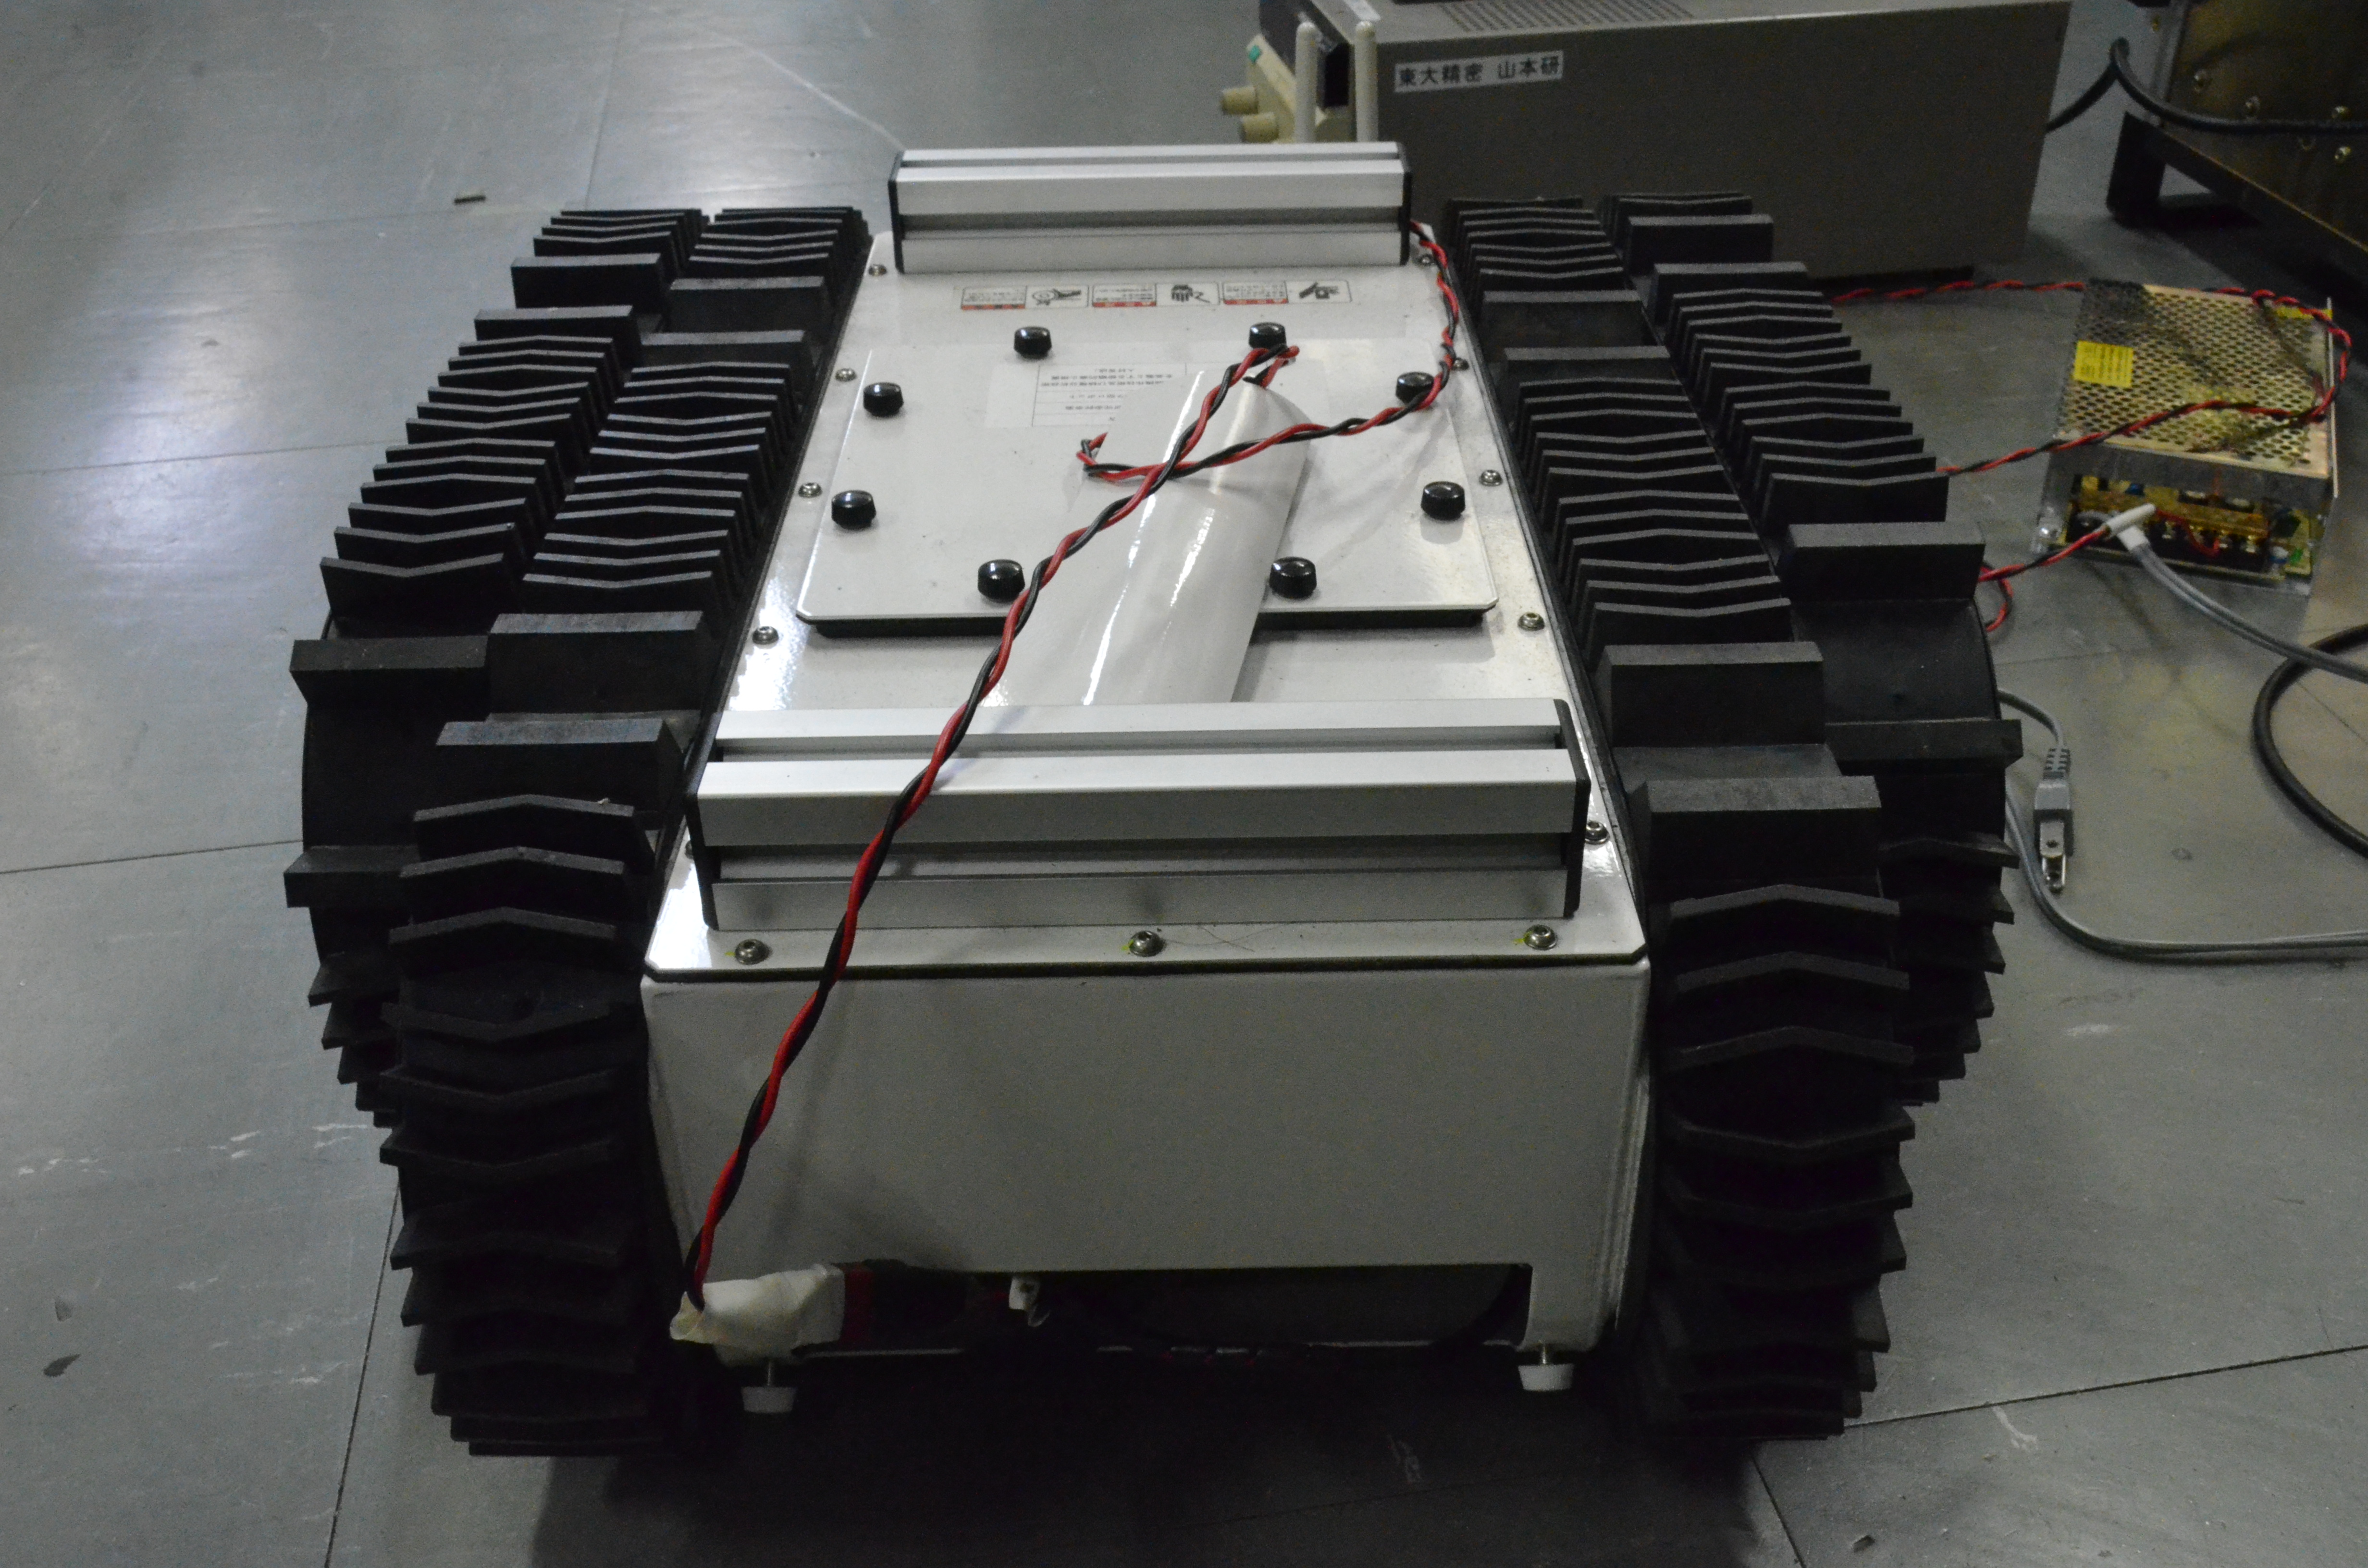
\includegraphics[width=0.6\linewidth]{Figs/topy_robot}
	\caption{Topy robot for real-world controller test setup.}
	\label{fig:topy_robot}
\end{figure}
After the theoretical analysis and model identification of the PlayStation-controller, the setup has been put to the test. At first, the controller has been connected to the computer to communicate with the Topy robot. The communication software was written in processing \cite{Fry2018} and is explained in a different section.\\ %TODO write about the software somewhere, reference here
\subsection{Latency}
The controller was successfully able to navigate the robot, if with a delay of roughly $700$ms. The commercial controller, that was developed for the Topy robot, also had a certain delay of almost $500$ms. This delay is the difference between the instant when the joystick is pushed forward, and the moment when the robot starts moving. The feedback methods that have been tested varied between a pure pitch feedback, a combined pitch and roll feedback and a current consumption feedback law. \\%TODO state the feedback laws and reference here
The effect and magnitude of the command latency, but also of the feedback latency can be seen in figure \ref{fig:real_P_scope_13_latency_plot} and \ref{fig:real_PID_scope_14_latency_plot}.

\begin{figure}[h!]
	\centering
	\includegraphics[width=1\linewidth]{Figs/real_P_scope_13_latency_plot}
	\caption{Command and behavior of Topy robot with P-controlled PlayStation controller.}
	\label{fig:real_P_scope_13_latency_plot}
\end{figure}


\begin{figure}[h!]
	\centering
	\includegraphics[width=1\linewidth]{Figs/real_PID_scope_14_latency_plot}
	\caption{Command and behavior of Topy robot with PID-controlled PlayStation controller.}
	\label{fig:real_PID_scope_14_latency_plot}
\end{figure}

In these figures, several interesting things have to be mentioned. First of all, the delay between sending the commands and receiving the consumed current value, which is then used as feedback value, is roughly $700$ ms. The delay between the received feedback value and the response of the distance sensor is much smaller and depends on the situation of the robot. When the robot starts to move, it takes some time until the current has built up, and the latency between the reference compression and actual compression is roughly $130$ ms for the P-controlled, and $430$ ms for the PID-controlled setup (see first red vertical lines). However, when the robot is stopped, the latency is $20$ - $30$ ms (second and third red lines).\\
In the first green lines, an external force has been applied to the robot, simulating an obstacle, which increased the consumed current and therefore also increased the desired feedback value. Again, the latency was of roughly $30$ ms. The second green lines is where the external force has been removed and the current dropped abruptly back to its normal value. The latency here was below $10$ ms.\\
Also indicated in figures \ref{fig:real_P_scope_13_latency_plot} and \ref{fig:real_PID_scope_14_latency_plot}, one can see that the feedback has been turned off when driving backwards (balck lines). However, in this scenario the feedback has been activated when standing still, ie. sending $0$ as driving speed. Since the robot is only sending the magnitude but not the direction of the current in the crawlers, the remaining current from the backward motion is fed back. This mode can easily be turned off, such that no feedback is felt when the robot is off. For reasons of completeness however, this has not been turned off and it is interesting to note, that the time between switching the command values and the reception of the feedback value has been reduced to roughly $50$ ms. \\
From these experiments one can conclude that the robot takes a long time to start driving, mainly due to internal implementation of the crawler control scheme. The total delay for this inital start-up is $820$ ms for the P-controlled and $1160$ ms for the PID-controlled version. The communication delay (joystick command and robot's reaction) is $40$ ms on average. The time between sending the joysticks commands and feeling the feedback is $240$ ms (P) and $280$ ms (PID). The full data has been gathered with an oscilloscope and can be seen in table \ref{tab:latency_table}.

\begin{figure}[h!]
	\centering
	\begin{tabular}{|l|c|c|c|c|c|c|c|c|}% Go | Stop | start pushing | let go | stop | back | stop| 
		\hline
	 	 & Start & Stop & Ext. force & No force & Stop & Back & Stop & Control\\ \hline \hline
		Joy-stick commands sent & 1.03 & 2.51 & - & - & 6.54 & 7.18 & 8.53 & P\\ 
		\hline
		Measured current in robot & 1.34 & 2.67 & 4.35 & 5.91 & 6.66 & 7.57 & 8.66 & P\\ 
		\hline
		Desired compression & 1.72 & 2.80 & 4.61 & 6.10 & 6.81 & - & 8.57 & P\\ 
		\hline
		Measured compression & 1.85 & 2.83 & 4.64 & 6.10 & 6.81 & - & 8.66 & P\\ 
		\hline \hline
		Joy-stick commands sent & 0.09 & 2.52 & - & - & 6.53 & 7.15 & 8.43 & PID\\ 
		\hline
		Measured current in robot & 0.26 & 2.66 & 4.44 & 5.76 & 6.66 & 7.26 & 8.55 & PID\\ 
		\hline
		Desired compression & 0.82 & 2.80 & 4.70 & 6.01 & 6.80 & - & 8.49 & PID\\ 
		\hline
		Measured compression & 1.25 & 2.83 & 4.75 & 6.02 & 6.82 & - & 8.67 & PID\\ 
		\hline
	\end{tabular}
	\caption{Latency table for sending joystick commands, current measured on the real robot, desired compression and measured compression. All values indicated in [s].}
	\label{tab:latency_table}
\end{figure}



\subsection{Real-Feel and Intuitiveness}
Despite the command delay, the feedback from the robot can be felt almost instantly in the user's palms. It is, as soon as the robot is moving forward, one can feel the current building up in the current consumption feedback mode for example. \\
The difference between the PID and P-controlled controllers is small, but can still be felt. In the PID-control scheme, one can feel an asymmetry between the left and right palms. This is due to the distance sensors that have different threshold values and the fact that the PID gains have been tuned for one side only. To avoid this asymmetry, it is recommended to identify different gains for the two sides or use sensors with more similar threshold values.\\
The proportional control scheme is already capable of giving an intuitive feedback of the robot's state. Especially since the feedback value is continuous and does not change much over time for all feedback modes. For these reasons, it seems appropriate to leave the controller P-controlled only.\\
\subsection{Stability}
Both control schemes are stable for various grips and feedback values, but in some cases one can feel and hear a slight instability in the PID-controlled setup. This suggests that the gains are not optimal and that they can further be tuned in future research. However, it is not possible to render the setup instable even when the user is deliberately trying to do so, acting as a non-passive element. 

\subsection{General Performance}
The overall performance evaluation of this controller is rather subjective. The output force of the SEA setup is much bigger than for the voice-coil implementation, as it has been foreseen in the design phase. Since the output force is distributed over the whole area of contact of the stimulators, the user technically feels a pressure instead of the force itself. However, one can call the feedback a pseudo-force as it has been shown in the previous research of this project \cite{Asada2016}. One important psychological aspect is the area of the stimulators. If they are too big, the pressure is much wweaker and the pseudo-force is too weak. If the area is too small, the feedback becomes punctual and the edges distort the feeling of the feedback, making it uncomfortable to use and anti-intuitive. In this controller design the stimulators have the right ratio between output force and area of contact.\\
Another psychological aspect is the direction of the feedback. This controller has an angle of roughly $ 115^\circ$ with respect to the operator's orientation. During operation the forces tend to push the palms outwards which is not entirely intuitive if one is expecting a force opposing the movement of the robot ($180 ^\circ$). This however depends strongly on the target application and the controller design can be well-suited for other environments.\\ %TODO state this somewhere (drones, bagger, car, etc.)

The biggest issue in this test setup though, is the delay of the command messages. In order to get an idea of the delay of the mechanical setup (the SEA implementation) the controller has also been tested in a purely simulated environment. This eliminates all potential delays in communication between robot and controller and the results and evaluation can be seen in the next section.

\subsection{Unity Simulation}
\begin{figure}[h!]
	\centering
	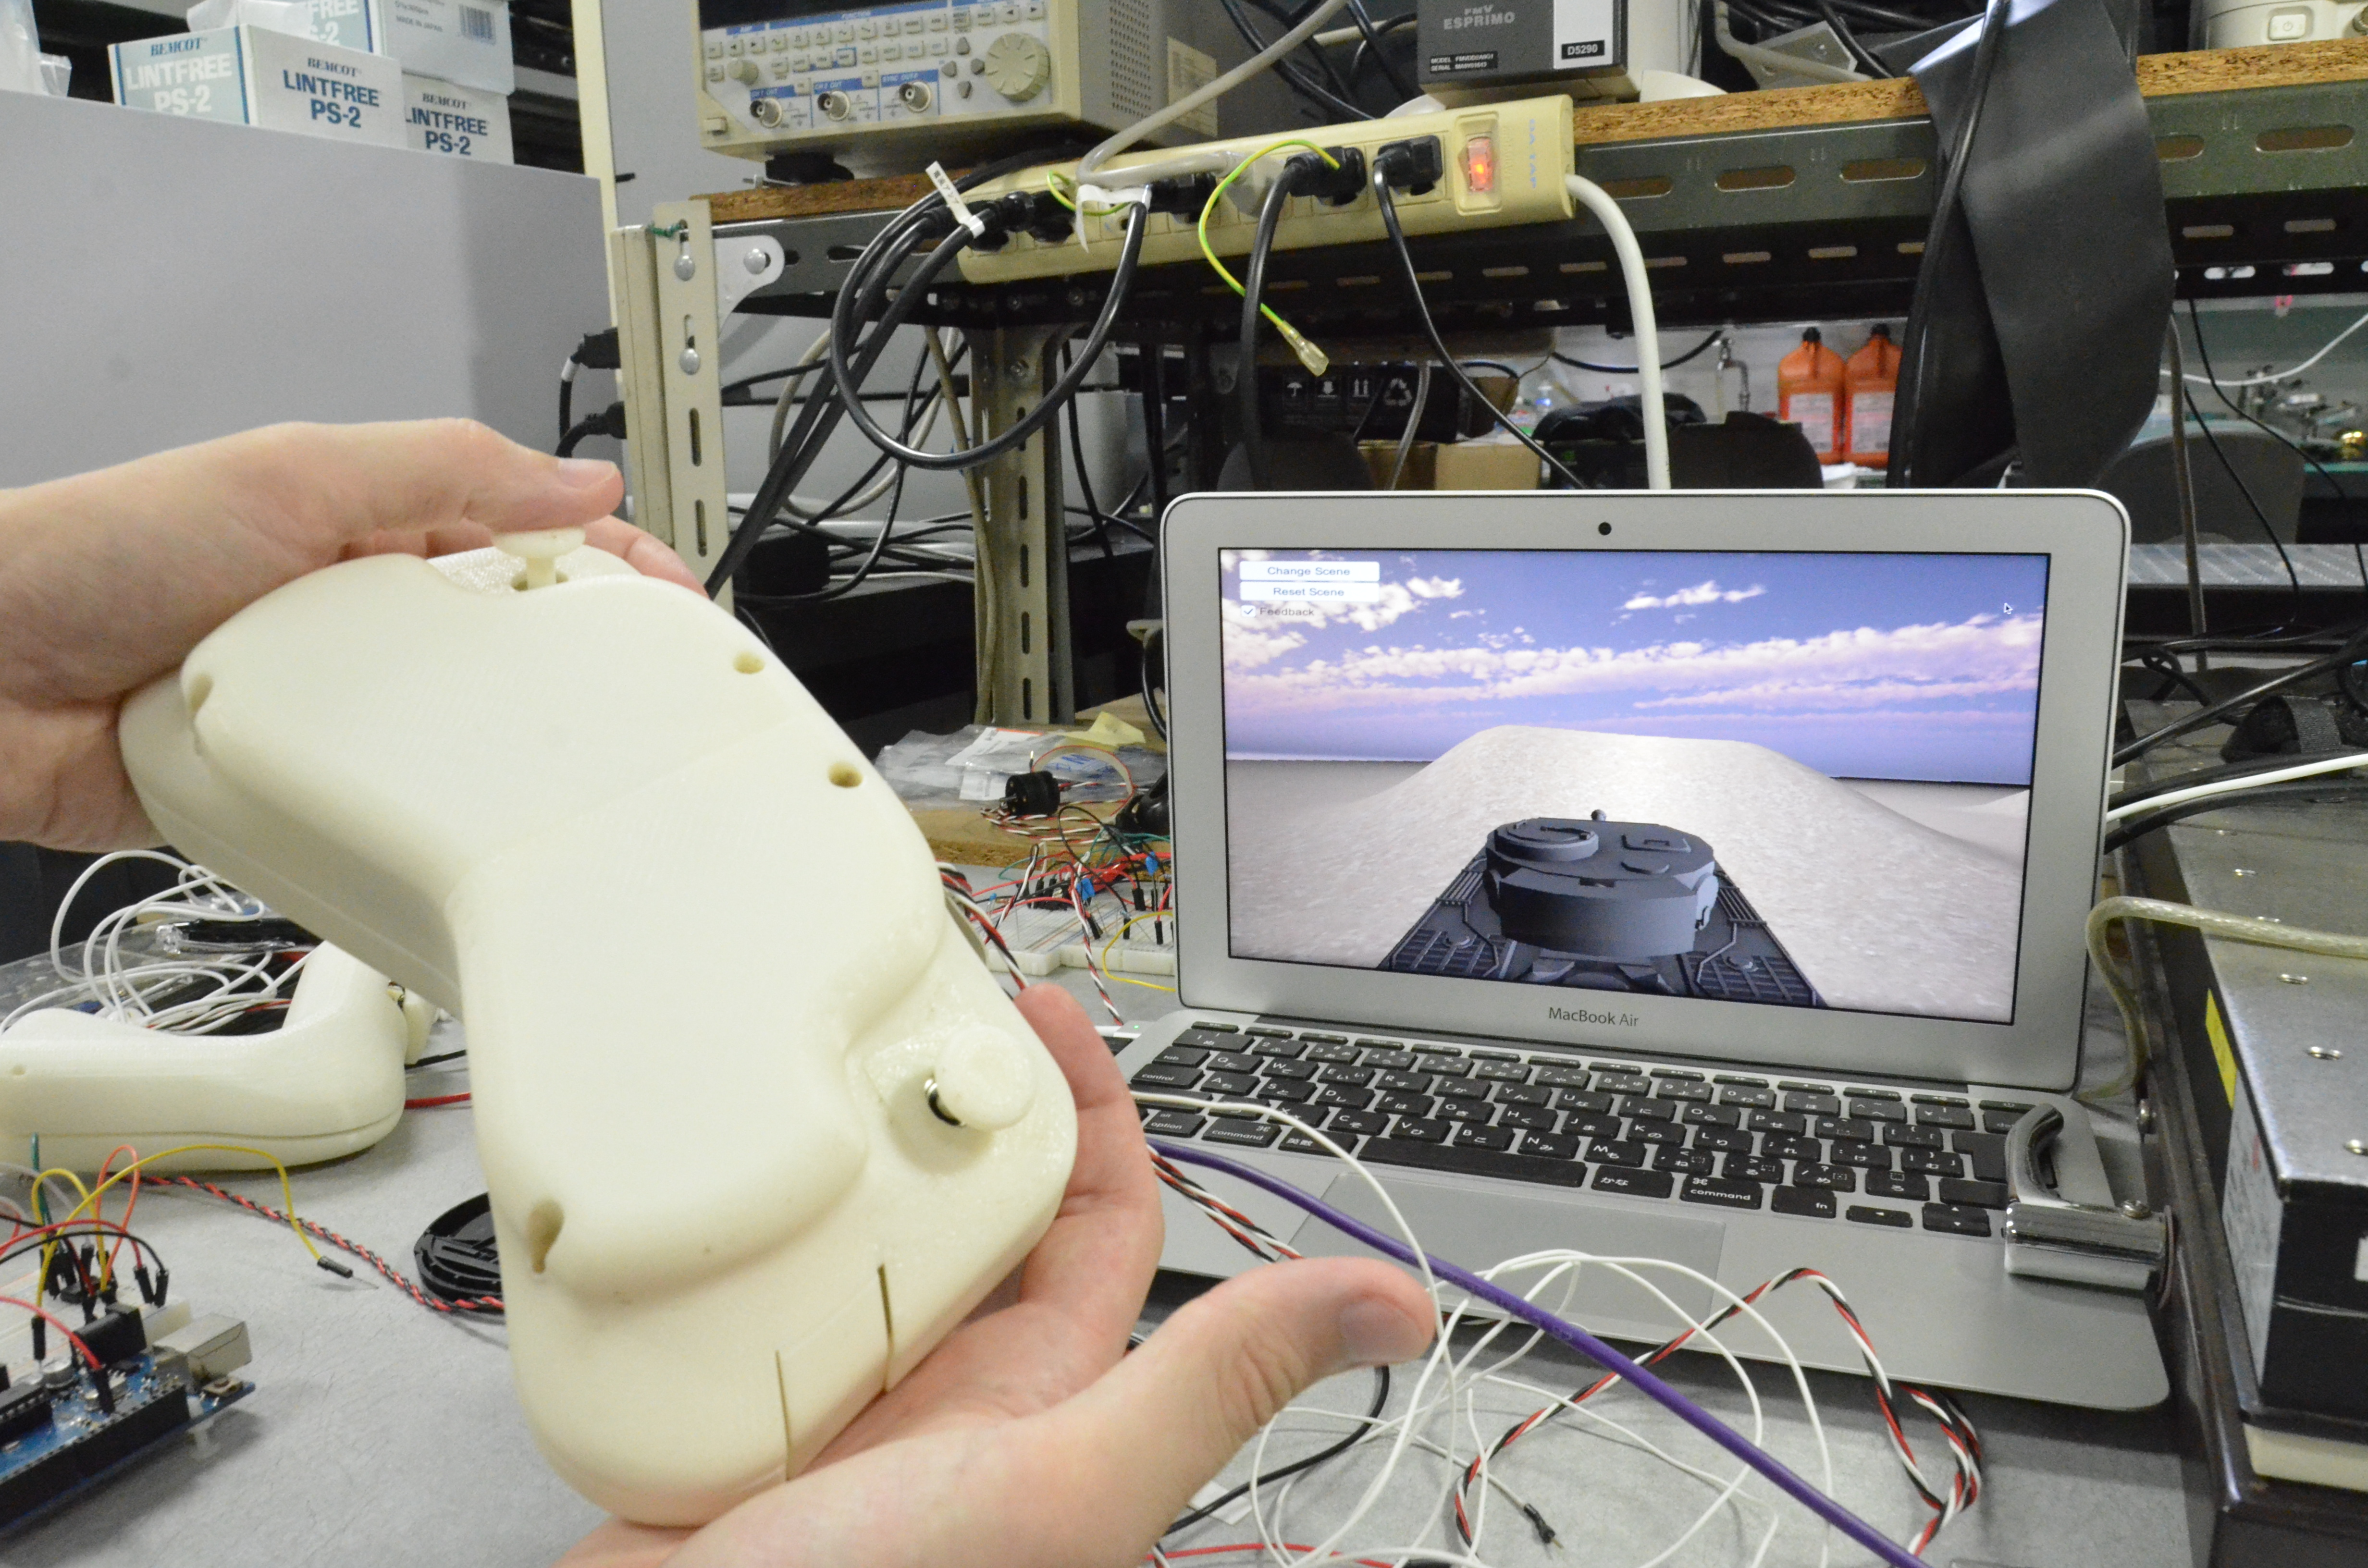
\includegraphics[width=0.6\linewidth]{Figs/unity_test_setup}
	\caption{Unity simulation test setup.}
	\label{fig:unity_test_setup}
\end{figure}
For testing the controller in the simulated world, the Unity program from the previous research of this project has been used. With minor modifications of the control software, the controller could be tested with different feedback for the two stimulators. This time, only the combined roll-pitch feedback law has been used.\\
Since all communication delays have been eliminated, the simulated tank reacted instantly to the user's command and its orientation angles is fed back. \\
There is no latency feelable, neither when sending the commands, nor when receiving the feedback. The real-feel of the controller is better than before and even the maximum output force could be achieved when driving over the steep slopes of the environment. The range of the output force is appropriate for the desired feedback. And obstacles or slopes can be felt individually and intuitively on both sides.\\
This simulation only test shows that the latency reported in the previous section does not stem from the implementation of the series elastic actuators and justifies the choice of this actuation system.\\

\subsection{Overall Evaluation of the PlayStation Controller}
Overall one can say that the controller has achieved the performance requirements stated in the beginning of the project. \\ %TODO maybe reference here
The advantages of using SEA's are mostly the increased maximum output force and the decreased weight (VCM's tend to be very heavy due to the magnets). A drawback however is the size of the controller. The controller has been designed with several margins for dimensions and distances, leading to this bulky setup. If necessary, the design can be optimized in a future work, which would result in a much smaller controller than the current design.\\
Both control schemes (SEA and VCM) are straightforward and the output force can be controlled easily.\\
The disadvantages of the SEA implementation are the control speed and reaction time of the mechanical setup. As it has been shown in both testing environments, the mechanical response time is not the bottleneck in this setup.\\
Even though the maximum output force is enough to give a good feedback, it can be further increased. The motors that are used currently are not capable of compressing the springs to their maximal deflection. Therefore it is enough, to switch out the motors to have a higher torque. But when doing so, it should be verified, that the control speed of the motors do not affect the overall response time.\\
From the psychological points of view, the only shortcoming is the direction of the feedback which is application-specific. For this reason, and in order to write and test a parameter choice framework for future research projects, based on the current findings, a second controller has been designed.\\


\section{Design Framework}
This section provides a guideline for important design parameter choices, if one wants to design a similar haptic feedback controller based on series elastic actuators. It is mainly based on the findings from the PlayStation controller but also includes the main results of the second controller, called pilot controller. \\
Since the design framework depends on the target application, it is assumed to use the controller for robots similar to the Topy robot.

\subsection{Software and Control Choices}
In order to introduce no latency for control commands, it is important to have a high communication speed with no delay. In the current Arduino setup, one can decrease the command delay by using interrupts for the joystick commands. For immediate feedback, one can implement a feedforward control scheme that is fed from the joystick's positions directly to the stimulators.\\
The bottleneck of this setup was the fixed communication frequency of the Topy robot of maximum $5$ Hz. Due to the small changes of the feedback value, this operation frequency is still acceptable. But if one expects a highly fluctuating feedback, a higher communication frequency has to be opted for.\\
The suggested control scheme is a normal proportional controller, mainly due to the fact that it is bothersome to fine-tune the PID gains.\\
For haptic applications, it is suggested to have at least a motor control rate of $1$kHz which is the limit for the Arduino. If one opts for higher control frequencies, it is recommended to switch to an Mbed device or similar devices.
%software and control

\subsection{Mechanical Parameters}
One of the first mechanical design choices is the design of the controller itself. The PlayStation like controller has been chosen for consistency with the previous research, but also for the fact that most conventional controllers are based on this design. It is not required to copy this design, which is why a different approach has been chosen for the second controller design.\\
The feedback direction is target-application specific and results from the design. For the desired application, it is recommended to have a direct movement opposing force, as it is the case for the pilot controller design.\\
The weight only plays a minor role and any weight seems to be fine as long as the operator is comfortable with handling the controller.\\

The target point of contact with the user's palm is between the Mars and Venus region %TODO reference hand terminology
. This area is sensitive enough and can have a typical indentation of $5$mm which needs to be taken into account when calculating the necessary stroke of the stimulator. The palm pads' areas should be around $5$ to $10$ cm$^2$.\\

Another important element is the spring system that can be chosen. It is recommended to have a symmetric arrangement with springs of equal spring constant. Also, it should be paid attention to symmetries when assembling the springs, to assure a linear behavior when compressing. The length of the springs does not seem to be very important, as long as the compression is constrained to the perpendicular axis only. Testing different deflections has shown that the target stroke must be achievable and that it is better to have a margin if one wants to change the motors used to increase the output force.\\
The spring coefficients can vary and tests between $2$ and $24$ N/mm have shown promising results. %TODO emphasize these tests or outcome, and reference somehow, link to results or data

The motors greatly influence the performance of the controller. The reduction ratio should be high enough to guarantee the target output force, while assuring the desired control speed. The target output torque can be used to calculate the output force approximately. But one should keep in mind that some energy is lost in friction and efficiency of the motor and gear assembly.
%mechanical (springs (length, size, arrangement), motors (speed/reduction, output torque), design (orientation, stimulators, etc.), weight)

\subsection{Electrical Parameters}
The electric components that have been used are mainly the potentiometer for the joysticks and the photoreceptors for distance sensing.\\
The photoreceptors have very different characteristics and all thresholds need to be identified individually. Furthermore, the output function is not linear for a big range of distances and the sensitivity also depends on the distance. If a high performance is expected from the controller, it is recommended to find a different solution or a better performing sensor.\\
Furthermore, it is recommended to filter the motor commands to convert the Arduino output PWM to a more steady voltage level, to protect the amplifiers from overfitting the signal.\\
Also, it was necessary to have a voltage follower (a simple operational amplifier with unitary gain) in order to reduce interfering effects on the distance sensors.
%electrical (sensors, joystick)

%say what parameters are important, how they affect the controllers, etc.
%say what i have found for my PS controller and what i can change

\section{Pilot Controller}
Based on the framework from the previous section, a new controller has been devised, mainly focusing on a different design and on a more optimal feedback direction.

\subsection{Working Principle (cam)}%TODO put text from april here
Has already been stated in April's monthly report.

\subsection{Design and Parameters}
When designing this controller, the design of an airplane yoke has been used as a model. Therefore it is from now on called pilot controller. In order to have a nice fit to the palms, the circumference has been chosen to be close to the airplane yokes or conventional car steering wheels. The joysticks' position is such that the stimulator touches the same area of the palm as in the previous controller and research (Venus and Mars area of the hand). This time the feedback direction is perpendicular towards the user, which ensures a more intuitive feeling for the desired application.\\
The most important parameters in this system are the length of the lever and the springs. For the prototype, the levers length has been fixed to roughly $100$ mm and a set of four springs with $1$ N/mm each have been used. Their length is $10$ mm and they have an allowable deflection ratio of $40$\%.\\
The stimulators area is kept almost the same with $7.5$ cm$^2$.\\
The motors play an important role again and for this design, the motors with the reduction gear of $33:1$ have been implemented.

When designing the rotational cam part, a spiral-like freeform has been drawn to keep the angle-to-distance ratio as linear as possible. The operational range of the motor shaft is $110 ^\circ$. It is, the full stroke of the lever can be achieved by rotating the motor shaft and the attached rotation cam by this angle.\\

The operational distance for the photoreceptors is between $11$ mm and $8$ mm. 
Again the operational range of the photoreceptors can be identified.

\begin{figure}[h!]
	\centering
	\begin{tabular}{|l|c|c|c|c|c|}
		\hline
		& Sensor reading & Distance & Sensor reading & Distance & Max output  \\
		& MAX (rest) & (rest) & MIN (compression) & (compression) & force \\ \hline \hline
		Left side & 800 & 11mm & 550 & 8mm & 12N \\ \hline
		%Right side & 870 &2.2mm & 700 & 8mm & 10.8N \\ \hline
	\end{tabular}
	\caption{Identified operational range for the photoreceptors in the pilot controller.}
	\label{tab:oper_range_pilot}
\end{figure}
%state the parameter choices that i have made based on previous findings
\subsection{advantages and disadvantages}%TODO is this really necessary or can i write it under design and parameters
%state advantages and disadvantages
\subsection{Analytical results}
%state analytical results (if available)
\subsection{Frequency Response Analysis}
Similar to the previous frequency response analysis, the controller has been tested when feeding a sine wave in the range of $1$ Hz up to $100$ Hz. The result for the P-controlled device can be seen in figure \ref{fig:pilot_bode_P02}

\begin{figure}[h!]
	\centering
	\includegraphics[width=0.6\linewidth]{Figs/pilot_bode_P02}
	\caption{Frequency response function of the P-controlled pilot controller.}
	\label{fig:pilot_bode_P02}
\end{figure}

The bode diagram resembles the one of the previous setup, with the main difference, that it seems to be shifted towards lower frequencies. The phase offset changes almost linearly from $45 ^\circ$ to $200 ^\circ$. Analogously, it is argued that the initial phase lag for low frequencies stems from the different filters that have been implemented in the same manner. Regarding the magnitude plot however, it is important to note that the resonance frequency is much lower, namely $4$ Hz.\\

In the current design of the pilot controller, the lever is roughly $100$ mm and has been fabricated using an $8$ mm thick poly-acetal plate. Due to the relative low thickness, the lever can deform and thus leads to an additional spring element in the system. Furthermore, the rotation cam is not coupled to the lever and thus cannot make pull it back in order to decrease the springs' compression, even if a negative voltage is applied. This leads to a lower overall performance and results in a lower resonance frequency.\\
In order to deal with this issue, it is recommended to preload the lever that pulls it back faster than normal, or couple the rotational cam with the lever.

\subsection{Pilot-Controller Testing}
%state real feel, latency, transparency and stability
\subsection{Outlook}
%state possible improvements for future work


\section{Discussion}	

\section{Conclusion}


\section{Outlook}



	
	%‚±‚±‚Ü‚Å
}

